% ACTIVE VOICE CHECK EVERYWHERE

\documentclass[12pt]{article}
\usepackage{amsmath}
\usepackage{amsfonts}
\usepackage[title]{appendix}
\usepackage{mathtools}
\usepackage{cite}
% to break urls: https://tex.stackexchange.com/questions/115690/urls-in-bibliography-latex-not-breaking-line-as-expected
\usepackage[hyphens]{url}
\usepackage{graphicx}
\usepackage{caption}
\usepackage{subcaption}
\usepackage{multirow}
\usepackage{draftwatermark}
\usepackage{pgffor}
\usepackage{alphalph}
% usually hyperref has to be the last package imported
\usepackage{hyperref}
%
\setlength\parindent{20pt}
\SetWatermarkText{Draft}
\SetWatermarkScale{10}
%
\newcommand{\beq}{\begin{equation}}
\newcommand{\eeq}{\end{equation}}
%\newcommand{\ber}{\begin{eqnarray}}
%\newcommand{\eer}{\end{eqnarray}}
\newcommand{\nn}{\nonumber}
\newcommand{\dd}[2]{\frac{d}{d{#2}}{(#1)} }
\newcommand{\pdd}[2]{\frac{\partial{{#1}}}{\partial{#2}}}
% define variables for \mupics command
\newcommand{\nhghaloesheight}{3.0cm}
\newcommand{\nhghaloeswidth}{0.19\linewidth}
\newcommand{\nhghalfwidth}{0.48\linewidth}
\newcommand{\nhgtotalheight}{4cm}
\newcommand{\nhgappwidth}{0.23\linewidth}
\newcommand{\nhgappheight}{2.2cm}
% mupics ends here
% filterloop starts here
\newcommand{\filterpics}[1]{
  \foreach \myvar in {0,...,31}{
    \begin{subfigure}[b]{2.2cm}
      \includegraphics[totalheight=2.0cm]{Figures/#1/filter_\myvar_channel_0.png}
      \caption{}
    \end{subfigure}
  }
}  
\begin{document}
% bib
\title{Elasticity imaging using a Convolutional Neural Network}
\author{Nachiket Gokhale\footnote{The author is very grateful to Paul Barbone (Professor, Mechanical Engineering, Boston University, Boston, MA, USA.) for patiently answering many questions about finite elements and for his constructive comments on an earlier version of this document. Conversations with Arnab Majumdar (ArcVisions, Kolkata, India), Michael Richards (Assistant Professor, Department of Biomedical Engineering, Kate Gleason College of Engineering, Rochester Institute of Technology, Rochester, NY, USA) and Mandar Kulkarni (Houston, TX, USA) are gratefully acknowledged and appreciated.}\\gokhalen@gmail.com\\Pune, India.}
\date{\today}
\maketitle
\abstract{We explore the application of a Convolutional Neural Network (CNN) using labeled data (supervised learning) to image the shear modulus field of an almost incompressible elastic medium in plane strain using data which consists of displacement or strains fields (or components thereof). This problem is important in medicine because the shear modulus of suspicious and potentially cancerous growths in soft tissue is elevated by about an order of magnitude as compared to the background of normal tissue. Imaging the shear modulus field therefore can lead to high-contrast medical images. Our prediction problem is as follows: \textit{Given a displacement or strain field (or its components), predict the corresponding shear modulus field}. Our CNN is trained using 2400 training examples consisting of displacement or strain fields (or components thereof) and a corresponding shear modulus field. We present encouraging results which warrant further research and show the promise of this methodology.}
\section{Introduction}
The shear modulus of palpable nodules (which can be thought of as abnormal and potentially cancerous growths in soft tissue) is approximately an order of magnitude higher than the stiffness of the background of normal glandular tissue \cite{paper:sarv1998}. See also figure (\ref{fig:shearmod}). It follows then, that imaging the shear modulus field of soft tissue results in a high-contrast imaging method because the elevated shear modulus of suspicious growths will stand out clearly against the lower shear modulus of the background of normal tissue. Elasticity Imaging is a broad term that refers to methods which image the shear modulus (or other mechanical properties) of soft tissue in various ways. See \cite{paper:gao1996,paper:parker2010,book:alamgarra2019,bookchap:oberaibarbone2019} for comprehensive reviews of the field.
%
\begin{figure}[!h]
   \centering
    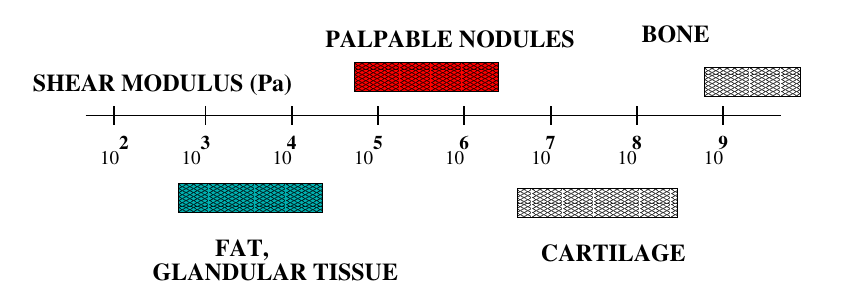
\includegraphics[totalheight=3cm]{Figures/shearmod.png}
  \caption{\label{fig:shearmod} Shear moduli of different types of soft tissue. Adapted from Figure (1) in \cite{paper:sarv1998}.}
\end{figure}
%
\begin{figure}[!h]
   \centering
    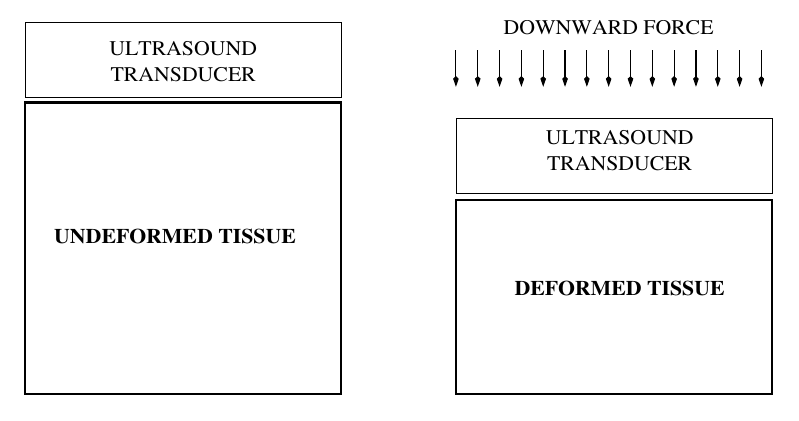
\includegraphics[totalheight=5cm]{Figures/prepostimage.png}
  \caption{\label{fig:prepostimage} Schematic figure showing medical image acquisition when soft tissue is being deformed using ultrasound imaging. The image taken on the left is referred to as the \textit{pre-deformation} image and the image on the right is the \textit{post-deformation image}.}
\end{figure}
%
\subsection{Steps involved in elasticity imaging}
Elasticity Imaging typically consists of the three steps of image acquisition, image registration, inverse problem solution. These steps are discussed in the following sections.
\subsubsection{Image acquisition} Images of soft tissue undergoing deformation due to applied excitation are acquired using various imaging modalities such as ultrasound or magnetic resonance imaging. While time dependent images can be acquired, we shall consider here only two images: a \textit{pre-deformation image} acquired before force is applied and a \textit{post-deformation image} acquired after force is applied. This process is shown in figure (\ref{fig:prepostimage}) for ultrasound imaging. Also see figure (2) in \cite{paper:konofagou2004}.
\subsubsection{Image registration} The goal in this step is to find a map which transforms the pre-deformation image into the post-deformation image. For every point in the pre-deformation image we aim to find its location in the post-deformation image. See figure (\ref{fig:registschematic}). This gives us the \textit{displacement field} between the two images. This displacement field is often referred to as the \textit{measured displacement field}.

Differentiating the displacement field with respect to spatial coordinates yields the strain field. If $u_x(x,y)$ and $u_{y}(x,y)$ are the $x$ and $y$ components of the displacement field, then the strain field is given by equation (\ref{eqn:straindef}). $\epsilon_{xx}$ and $\epsilon_{yy}$ are referred to as \textit{axial strains}. $\epsilon_{xy}$ is the \textit{shear strain}.
\beq
\label{eqn:straindef}
\epsilon_{xx} = \pdd{u_{x}}{x} \qquad \epsilon_{yy} = \pdd{u_{y}}{y} \qquad \epsilon_{xy} = \frac{1}{2}\Big(\pdd{u_{x}}{y} + \pdd{u_{y}}{x}\Big)
\eeq
See \cite{paper:richards2009,paper:gokhale2004,paper:pellot-barakat2004} for minimization based approaches for computing the displacement field. See \cite{paper:ophir1991,paper:ophir1996,paper:alam1998} and references therein for cross-correlation based approaches. In our work, we generate displacement fields from known shear modulus fields using the finite element method \cite{book:hugheslinear,book:fishbelytschko} and add appropriate noise to mimic the noise when displacement fields are computed from experimentally acquired images. See figure (\ref{fig:exampdispstrain}) for examples of displacement and strain fields computed using FyPy \cite{misc:fypy}.
%
\begin{figure}[!h]
  \centering
  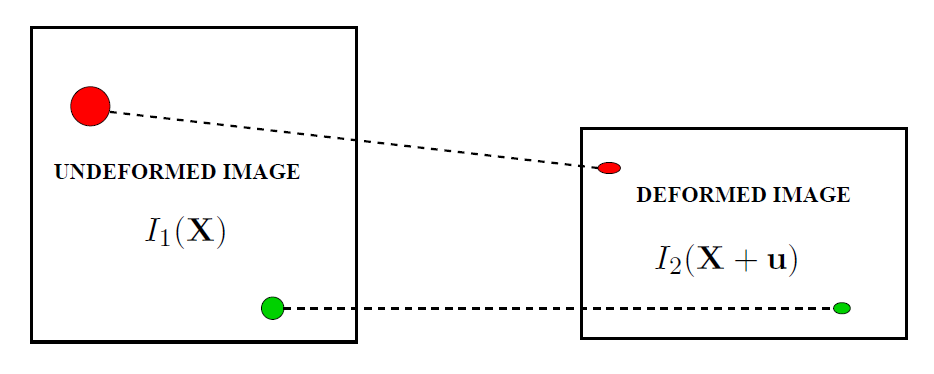
\includegraphics[totalheight=4cm]{Figures/regist.png}
  \caption{\label{fig:registschematic} A schematic figure of image registration. For the red and green points in the pre-deformation image on the left we aim to find their location in the post-deformation image on the right. Doing this for every point in the pre-deformation image yields a displacement field.}
\end{figure}
%
\begin{figure}[!h]
  \centering
  %
  \begin{subfigure}[c]{\nhghaloeswidth}
    \centering
    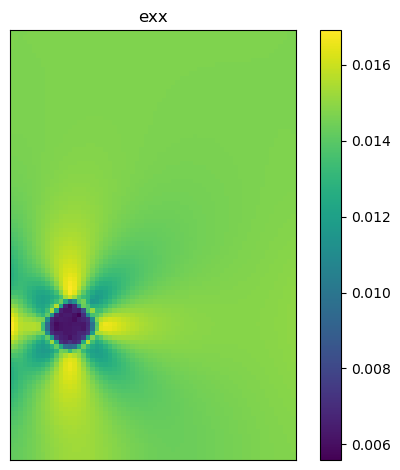
\includegraphics[totalheight=\nhghaloesheight]{Figures/dispstrainfields/exx.png}
    \subcaption{$\epsilon_{xx}$}
  \end{subfigure}
  %
  \begin{subfigure}[c]{\nhghaloeswidth}
    \centering    
    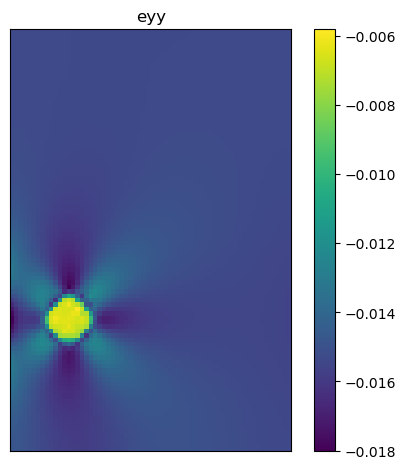
\includegraphics[totalheight=\nhghaloesheight]{Figures/dispstrainfields/eyy.png}
    \subcaption{$\epsilon_{yy}$}
  \end{subfigure}
  %
  \begin{subfigure}[c]{\nhghaloeswidth}
  \centering    
    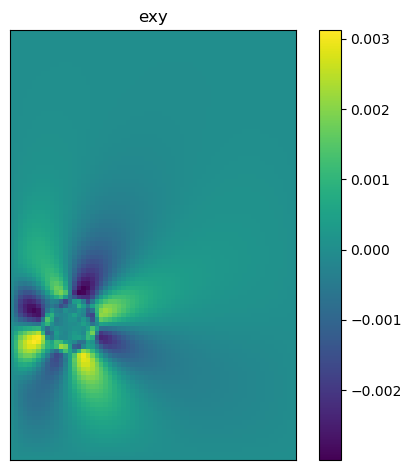
\includegraphics[totalheight=\nhghaloesheight]{Figures/dispstrainfields/exy.png}
    \subcaption{$\epsilon_{xy}$}
  \end{subfigure}
  %
  \begin{subfigure}[c]{\nhghaloeswidth}
  \centering    
    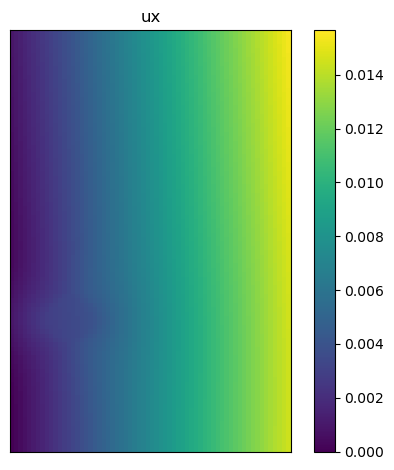
\includegraphics[totalheight=\nhghaloesheight]{Figures/dispstrainfields/ux.png}
    \subcaption{$u_{y}$}
  \end{subfigure}
  %
  \begin{subfigure}[c]{\nhghaloeswidth}
      \centering
    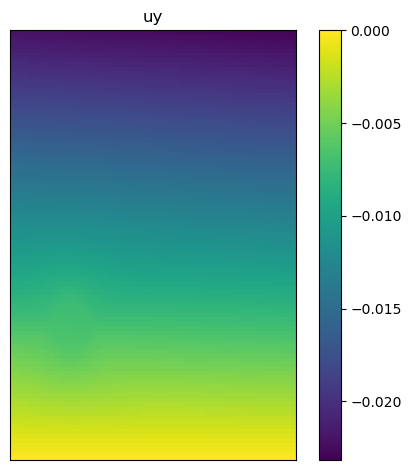
\includegraphics[totalheight=\nhghaloesheight]{Figures/dispstrainfields/uy.png}
    \subcaption{$u_{y}$}
  \end{subfigure}
  \caption{\label{fig:exampdispstrain} Examples of displacement and strain fields.}
\end{figure}
\subsubsection{Inverse problem solution} The goal in this step is to infer the spatial distribution of the shear modulus from the displacement field. This is called an \textit{inverse problem} because the classical boundary value problem in linear elasticity (referred to as the \textit{forward problem}) is to determine the displacement field given the shear modulus field, the Poisson's ratio field and suitable boundary conditions. See \cite{book:hugheslinear,book:fishbelytschko} for further details. The approaches for inverse problem solution can be divided into two categories: direct and iterative. These are discussed in the subsequent sections.
\subsubsection{Direct approach} Direct approaches involve solving a partial differential equation (PDE) to obtain the distribution of shear modulus directly: see \cite{paper:raghavan1994,paper:barboneadjwt,paper:albocher}. The coefficients of this PDE depend on the measured displacement field. Such approaches are fast and work well when the measured strain field is completely known and has low noise.
\subsubsection{Iterative approach} Iterative approaches \cite{paper:oberai2003,paper:gokhale2008,paper:kalle1996,paper:doyley,paper:goenezen2011} involve guessing a distribution for the shear modulus, solving a linear elasticity forward problem to obtain the predicted displacement field, computing the value and the gradient (and/or Hessian) with respect to the shear modulus of an objective function which consists of a user specified norm of the difference between the predicted displacement field and the measured displacement field, and updating the guessed shear modulus distribution using a suitable optimization procedure such as a modified Newton Raphson scheme as in \cite{paper:doyley} or the BFGS scheme as in \cite{paper:gokhale2008,paper:goenezen2011}. Such approaches are typically slower than direct methods, since they require the solution of approximately $50$ to $100$ forward problems, but have the ability to handle incomplete data and complex nonlinear material models such as hyperelasticity.
\subsubsection{Solving the inverse problem with CNNs}
We believe that solving the inverse problem with CNNs can combine the best characteristics of the direct and iterative approaches. The CNN based approach can yield a quick answer (once time has been spent up front to train the CNN), can accommodate complex constitutive relations, can work with incomplete data (e.g. only a single component of a displacement field) and can work with noisy data. On the other hand, if data which is unlike what the CNN has been trained on is seen, then the performance of the CNN will degrade. We also note that CNNs do not predict a perfect result in the absence of noise, unlike traditional direct or iterative methods. Finally, we note here that we expect determining multiple material parameters e.g. a linear and a non-linear parameter for hyperelasticity as in \cite{paper:gokhale2008}or both the Lam\'e parameters for compressible elasticity from the same set of images to be challenging.
\section{\label{sect:probsetup}Problem setup for data generation}
The displacement or strain field data required for the CNN is generated using a linear finite element solver named FyPy (\textbf{Fy}nite Elements in \textbf{Py}thon) \cite{misc:fypy}. We refer the reader to \cite{book:hugheslinear,book:fishbelytschko,book:segelmathcont} for details about the boundary value problem of linear elasticity and its solution using finite elements. Both displacements and material properties are interpolated bilinearly. The problem geometry is shown in figure (\ref{fig:bc}). Plane strain is assumed. The length (in the $x$ direction) is $1.0$ unit. The breadth (in the $y$ direction) is 1.5 units. Both degrees of freedom are constrained at the pin and only the $y$ degree of freedom is constrained at the roller. The background shear modulus is $\mu_{back}=1.0$ unit. The Poisson's ratio is a constant and is set to $0.49$. Selective reduced integration is used to avoid mesh locking \cite{book:hugheslinear} because the Poisson's ratio of $0.49$ renders the medium almost incompressible. The shear modulus of inclusions is a constant and is a random number ranging from $\mu_{min}=2.0$ to $\mu_{max}=5.0$. There are no homogeneous examples. The radius of the inclusion is a random number ranging from $0.05$ to $0.15$. There are either one, two or three inclusions in the data used to train CNN1 and CNN2 and there is exactly one inclusion in the data used to train CNN3. The parameters of the three networks are are listed in table (\ref{table:cnnparams}).

$4000$ displacement and strain images are generated and are split into $2400$ training examples, $800$ validation examples and $800$ test examples. The input data is scaled by the absolute maximum over all components. When noisy data is used, we add zero mean additive Gaussian noise in the strain or displacement data such that the signal to noise ratio ($\text{SNR}_{\text{dB}}$) is 40dB according to equation (\ref{eqn:snr}). We do not train CNNs with noisy data. Training of the CNN is always carried out on noiseless data and noisy data is given to the CNN as input.
\begin{subequations}
\begin{align}
  \text{SNR}_{\text{dB}} &= 20\log_{10}{\Bigg (}\frac{\|\text{signal}\|_{2}}{\|\text{noise}\|_{2}}{\Bigg )} \label{eqn:snr} \text{ where, }\\
  \|\mathbf{x}\|_{2} &= \sqrt{x_{1}^{2}+\cdots+x_{n}^2}  \text{ is the Euclidean norm.}   \label{eqn:eucnorm}
\end{align}
\end{subequations}  
% Noise details
%
\begin{figure}[!h] 
   \centering
    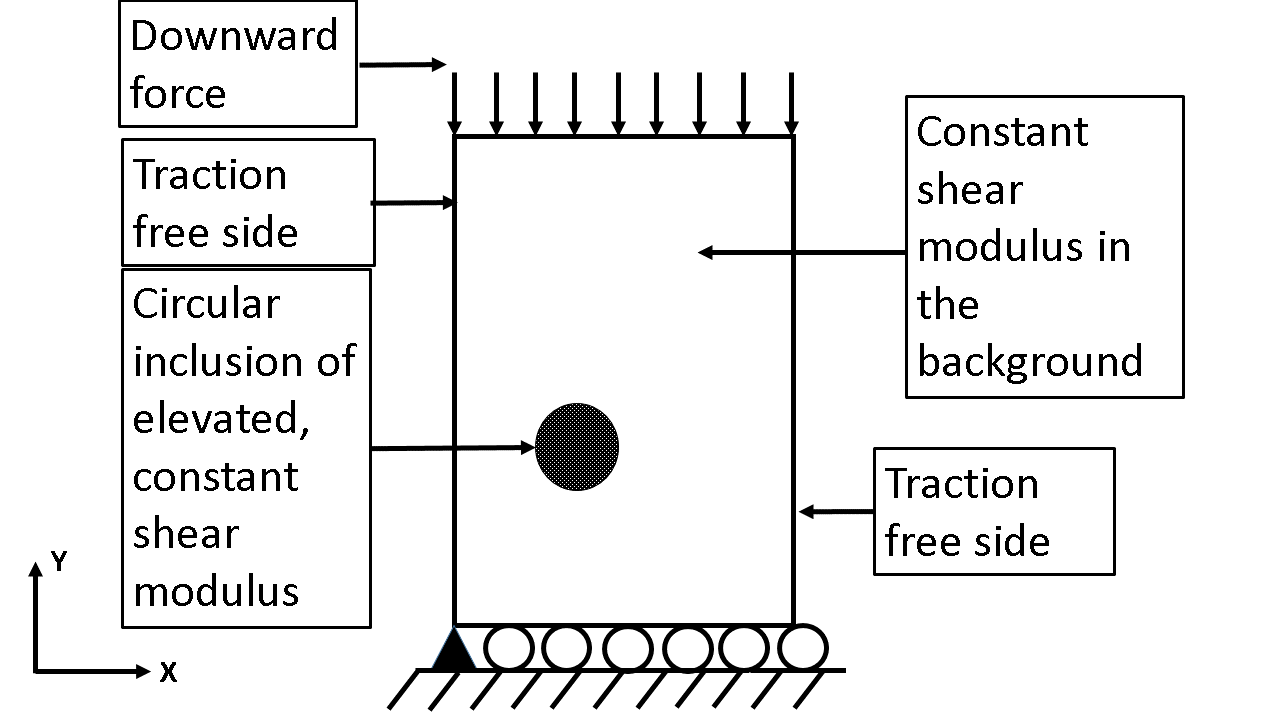
\includegraphics[totalheight=5cm]{Figures/bc.png}
  \caption{\label{fig:bc}Boundary conditions and material properties used in this work. }
\end{figure}
%
\section{Neural network architecture}
\subsection{Review}
In recent years, neural networks have been applied to various applications such as image classification \cite{paper:hinton2017}, hand written digit recognition \cite{paper:kulkarni2018}, solving differential equations and symbolic integration \cite{misc:lample2019}, solving complex partial differential equations such as the Navier-Stokes equation \cite{misc:anandkumar2020}, self-driving cars \cite{misc:agnihotri2019,misc:nvidiaselfdriving2016}, chaos \cite{paper:pathak2018}, natural language processing \cite{misc:googlenlp}, face recognition \cite{conf:taigman2014} and playing board games such as chess \cite{paper:alphazero}. Several effective Machine Learning frameworks such as Google's TensorFlow \cite{misc:tensorflow} (which we use in this work), Facebook's PyTorch \cite{incollect:pytorch}, Scikit-Learn \cite{paper:scikit-learn} are freely available. See \cite{misc:compdeep} for a complete list. We do not cover the theory of neural networks in this work. We refer the interested reader to \cite{book:aggarwal,book:goodfellow,book:chollet,misc:cs231n,misc:andrewng,misc:udemy} and references therein for detailed information about neural networks.
\subsection{Neural networks and elasticity imaging}
Given the success achieved by neural networks on the wide variety of applications cited in the previous section, it is natural to explore the application of neural networks to the inverse problem of elasticity imaging and several recent efforts \cite{paper:pateloberai2019,misc:gu2020,paper:hoeriginsana2016} have done so. In \cite{paper:pateloberai2019}, the authors use a convolutional neural network to classify specimens into elastically heterogeneous or elastically nonlinear. In \cite{paper:hoeriginsana2016}, the authors use a neural network to estimate strains and stress and then calculate elastic parameters. In \cite{misc:gu2020}, the authors use a neural network which predicts elasticity distributions using residual force maps to update the weights of the neural network.

In contrast, in this work we compute the shear modulus field from the displacement or strain field using a CNN. There are no physical constraints involved in our work. It is purely a mapping problem from the space of displacement or strain fields to the space of the shear modulus fields. The input data for our CNN is a set of strain or displacement fields or components thereof. For each input there is a known corresponding target shear modulus field. Starting from an initial random guess of the weights, the CNN predicts shear modulus fields, compares them with the target fields to compute the loss function and its gradient with respect to the weights of the neural network. The weights are updated using the gradient in an appropriate optimization algorithm. Thus the CNN learns weights for its filters and other parameters. Using this learned information, the CNN is able to predict a shear modulus field from the input data of strain or displacement fields. Figure (\ref{fig:schematic_inv}) shows the mapping of a displacement field to a shear modulus field.\\
\subsection{Need for neural networks}
At this point, it is worth asking the questions: Are neural networks really necessary? Would a brute-force algorithm suffice?.

Consider the following algorithm to solve the elasticity imaging problem.
%
\begin{enumerate}
\item{Let there be $n_{nodes}$ nodes used to discretize the shear modulus and displacement fields.}
\item{Let the shear modulus at each node be allowed to take $n_{\mu}$ discrete values between the minimum shear modulus $\mu_{back}$ and the maximum shear modulus $\mu_{max}$.}
\item{Solve and store displacement fields corresponding to every possible discrete shear modulus field.}
\item{When an unknown displacement field is encountered, find the closest displacement field from step (3) and output the corresponding shear modulus field as the answer.}
\end{enumerate}

The problem with the above algorithm is that the storage required in step (3) and the search space in step (4) is beyond enormous. There are ${n_{\mu}}^{n_{nodes}}$ possible shear modulus fields. This is an enormous number. To see this, take a concrete example: consider $n_{nodes}=1000$ and $n_{\mu}=10$. Then there are $10^{1000}$ possible shear modulus fields. We need an algorithm to search the large search space efficiently, and hence, the need for neural networks.
%
\begin{figure}[!h]
   \centering
    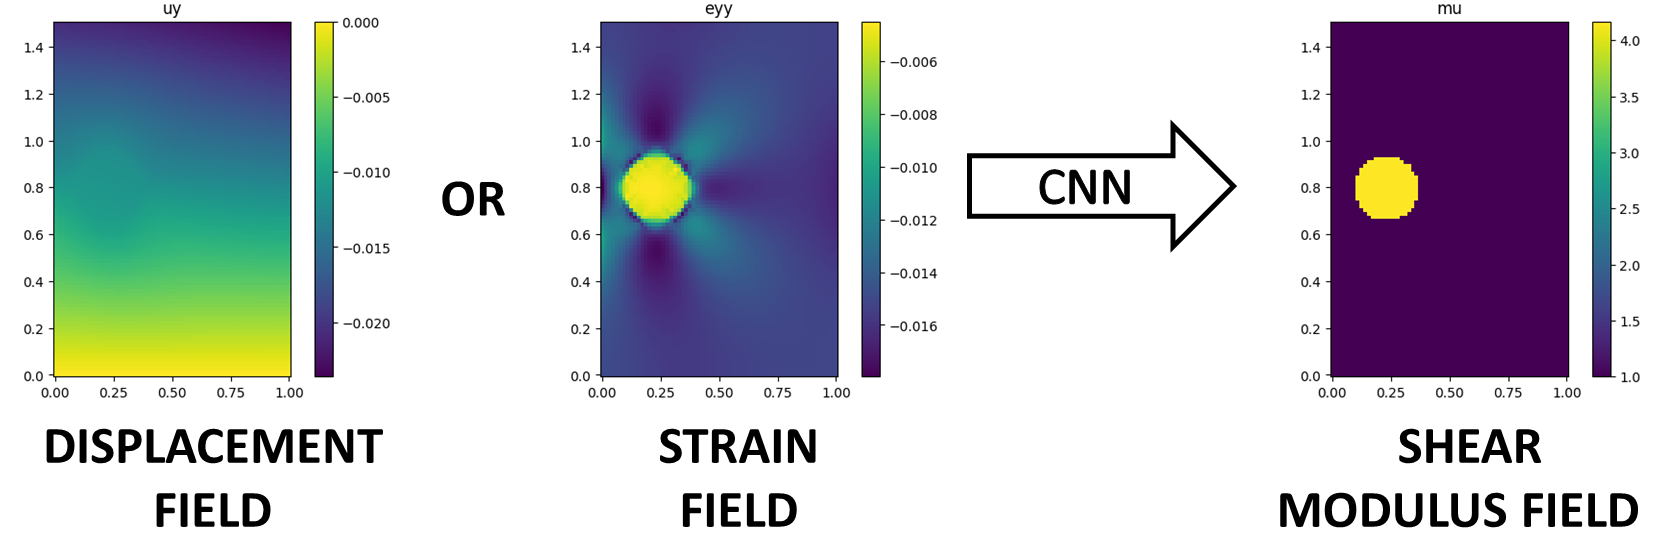
\includegraphics[totalheight=5cm]{Figures/schematic_inv/schematic_inv.png}
  \caption{\label{fig:schematic_inv} Solving the inverse problem using CNNs. The displacement or strain field (or components thereof) are mapped by the CNN into a shear modulus field.}
\end{figure}
%
\subsection{\label{sect:cnnarch} CNN architecture used in this work}
Figure (\ref{fig:typical_cnn}) shows the architecture of the CNN we use in this work. We implement this architecture in TensorFlow. The parameters of the layers are given in table (\ref{table:cnnlayerparams}).

The first dimension '?' represents the number of examples to be processed for training, validation or testing. Thus, the first training example's input data is a three dimensional array and can be accessed using the indices $[0,:,:,:]$ (using Numpy \cite{paper:numpy} notation) and similarly for the others. The second and third dimensions represent the number of nodes in the $y$ and $x$ direction respectively.

The last dimension represents the number of channels in the image. In color image-processing the number of channels is typically $3$, one channel each for the three colors red, green and blue (RGB). In our case, the number of channels is the number of components of the displacement or strain field used in our problem. If we use three independent components of the strain field $\epsilon_{xx},\epsilon_{yy},\epsilon_{xy}$ then the number of channels is $3$. If we use only a single component of the strain field, say $\epsilon_{xx}$ only, then the number of channels is $1$.
Since we are working with almost incompressible linear elasticity:
\begin{align}
  \epsilon_{xx}+\epsilon_{yy}\approx{0} \implies \pdd{u_x}{x} + \pdd{u_y}{y} \approx{0}.
\end{align}
In addition, in our problem setup, $\epsilon_{xy}\approx{0}$ almost everywhere. This implies that there is only one independent component in displacements and strains. We choose $u_y$ and $\epsilon_{yy}$ as the independent components and we restrict our attention to only single channel images which represent either $u_y$ or $\epsilon_{yy}$.

Finally, we note that the \textit{loss function} is \textit{mean squared error} and the optimizer is \textit{Adam} \cite{misc:kingma2017adam} with default TensorFlow settings. No regularization or dropout is used.  Each CNN has approximately $3.35$ million trainable parameters. After training, the model with the best validation loss is chosen to make predictions.
%
\begin{center}
\begin{table}
  \centering
  \begin{tabular}{|c|c|c|}
    \hline
    \multirow{2}{*}{CNN Name} &  \multirow{2}{*}{Training data}           & \multirow{2}{*}{Prediction data}\\
                              &                                           &  \\
     \hline
     \multirow{3}{*}{CNN1}    &  $\epsilon_{yy}$                           &  \multirow{3}{*}{$\epsilon_{yy}$ + 40dB noise}\\
                              &  noiseless                                & \\
                              &  1-3 inclusions                           &\\
     \hline
     \multirow{3}{*}{CNN2}    &  $u_{y}$                                   & \multirow{3}{*}{$u_{y}$ + 40dB noise}\\
                              &  noiseless                                & \\
                              &  1-3 inclusions                           &\\  
     \hline
     \multirow{3}{*}{CNN3}    &  $\epsilon_{yy}$                           & \multirow{3}{*}{$\epsilon_{yy}$ + 40dB noise}\\
                              &  noiseless                                & \\
                              &  1 inclusion                              & \\

    \hline
  \end{tabular}
  \caption{\label{table:cnnparams} Table of CNNs trained and their parameters. All CNNs use the twisted tanh [0.75,5.25] activation function (see section (\ref{sect:outputact})). CNN1 and CNN2 have the same true shear modulus fields. The shear modulus fields for CNN3 are different.}
\end{table}
\end{center}
%
\subsubsection{\label{sect:outputact} Output layer activations}
% 
\begin{subequations}
\begin{align}
f(x) &= &\ln(1+\exp(x)) \qquad &\text{softplus activation}\label{eqn:softplus}\\
f(x) &= &\frac{1}{1+\exp(-x)} \qquad &\text{logistic activation} \label{eqn:logistic}\\
f(x) &= &\tanh(x) \qquad &\text{tanh activation} \label{eqn:tanh}\\
%\text{softplusmin activation} \qquad f(x) &=& \min(\ln(1+\exp(x)),1.0)\label{eqn:softplusmin} \\
f(x) &= &\tanh(x) + 0.01x \qquad &\text{twisted tanh activation} \label{eqn:twisttanh}
\end{align}
\label{eqn:activations}
\end{subequations}
%
\begin{figure}[!h]
  \centering
  %
  \begin{subfigure}[t]{\nhghalfwidth}
    \centering
    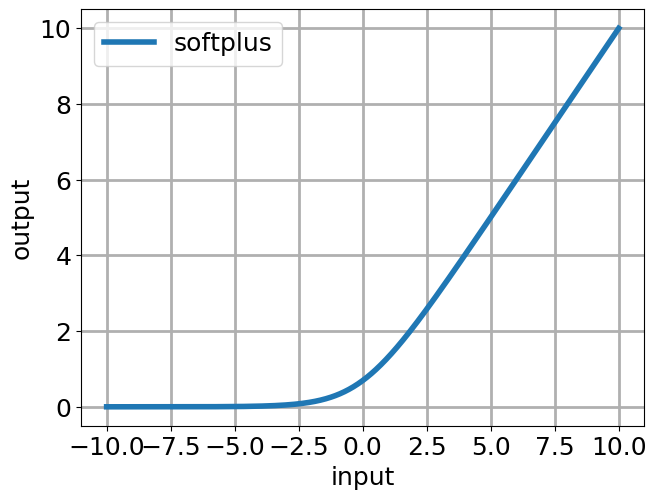
\includegraphics[width=4cm]{Figures/scripts/softplus.png}
    \subcaption{softplus}
  \end{subfigure}
  %
  \begin{subfigure}[t]{\nhghalfwidth}
    \centering
    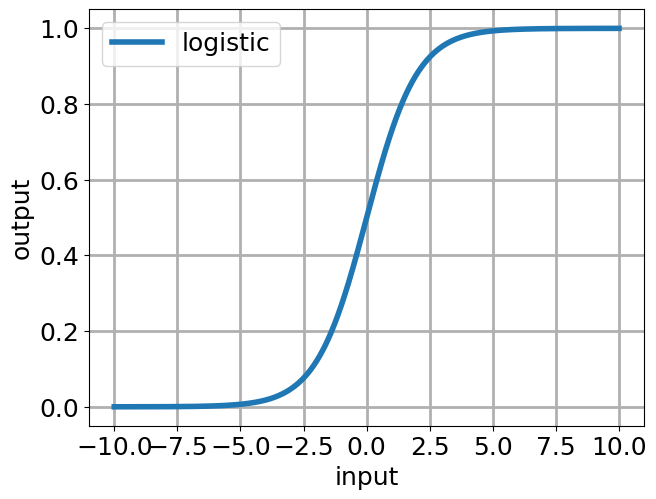
\includegraphics[width=4cm]{Figures/scripts/logistic.png}
    \subcaption{logistic}
  \end{subfigure}
  %
  \begin{subfigure}[t]{\nhghalfwidth}
    \centering   
    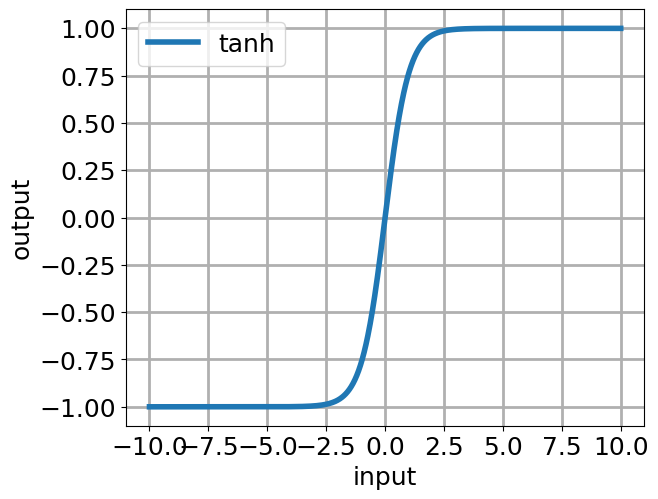
\includegraphics[width=4cm]{Figures/scripts/tanh.png}
    \subcaption{tanh}
  \end{subfigure}
  %
  \begin{subfigure}[t]{\nhghalfwidth}
    \centering
    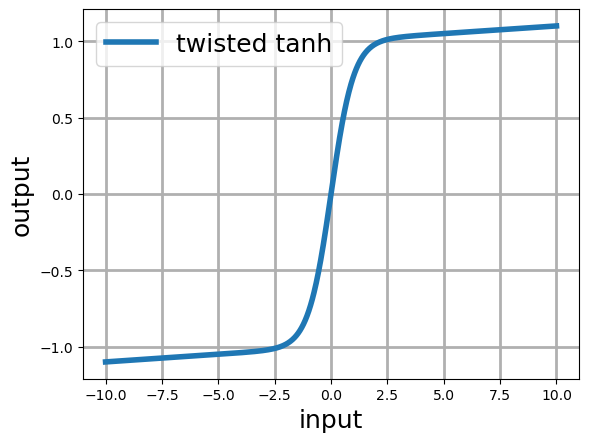
\includegraphics[width=4cm]{Figures/scripts/twistedtanh.png}
    \subcaption{twisted tanh}
  \end{subfigure}
  %
\caption{\label{fig:activations} Graphs of activation functions for equations (\ref{eqn:softplus}-\ref{eqn:twisttanh}).}
\end{figure}
%
We consider the functions given in equations (\ref{eqn:softplus}-\ref{eqn:twisttanh}) as activation functions for the output layer and choose the twisted tanh function, equation (\ref{eqn:twisttanh}), as the output layer activation. All our work is carried out using the twisted tanh activation function, unless specified otherwise.

The softplus activation function (\ref{eqn:softplus}) has range $(0,\infty)$ and thus it respects the physical positivity constraint on the shear modulus: $\mu(x)>0$ for reasonable materials \cite{book:segelmathcont}. The drawback of the softplus activation function is that it produces regions in which the shear modulus is very close to zero. We call such regions \textit{haloes}. See table (\ref{table:muminmax}) and figure (\ref{fig:haloes}).

We seek to avoid this problem by using the logistic and tanh activation functions, given by equations (\ref{eqn:logistic}) and (\ref{eqn:tanh}) respectively, whose range is limited to $(-1,1)$. Hence, the training data must be scaled such that it lies in the interval $(-1,1)$. This requires prior knowledge of the maximum and minimum value of the shear modulus, denoted by $\mu_{lower}$ and $\mu_{upper}$, to scale the training data using a linear transformation such that the interval $[\mu_{lower},\mu_{upper}]$ is mapped linearly to the interval $[-1,1]$. However, we find that as noted in \cite{bookchap:lecun98b}, the gradient of the logistic (\ref{eqn:logistic}) and tanh (\ref{eqn:tanh}) functions vanishes as we go farther away from zero. This causes the weights to get stuck and as a consequence the neural network does not learn.

To avoid this we add, as noted in \cite{bookchap:lecun98b}, a \textit{twisting term} $0.01x$ to the the tanh activation, equation (\ref{eqn:tanh}, to get the twisted tanh activation function, given by equation \ref{eqn:twisttanh}. The addition of the twisting term ensures that the gradient of the twisted tanh function does not vanish far away from zero. While the addition of the twisting term changes the range of the tanh function from $(-1,1)$ to $(-\infty,\infty)$, it is seen that in practice that the predictions of the neural network when rescaled lie only slightly outside the interval $[\mu_{lower},\mu_{upper}]$. This is seen in table (\ref{table:muminmax}).

We note that, when we write: ``twisted tanh $[\mu_{lower},\mu_{upper}]$'' we mean that we are using the twisted tanh activation function with the input data being scaled such that the interval $[\mu_{lower},\mu_{upper}]$ is mapped linearly to $[-1,1]$. The true range of the shear modulus for all the examples in this work is $[1.0,5.0]$ as noted before in section (\ref{sect:probsetup}).

\subsection{\label{sect:compsofttanh} Comparison: softplus and twisted tanh}
We now define the scaled error for the $i^{th}$  test example $\zeta_{i}$ and the average scaled error $\zeta_{ave}$ as
\begin{subequations}
  \begin{align}
  \zeta_{i} &\coloneqq \frac{\|\mu^{i,predicted} - \mu^{i,true}\|_{2}}{\|\mu^{i,true}\|_{2}}  &\label{eqn:scalederror}\\
  \zeta_{ave} &\coloneqq \frac{\sum_{i=1}^{n_{test}}\zeta_{i}}{n_{test}} &\label{eqn:averagescalederror}
  \end{align}
\end{subequations}
where $\mu^{i,predicted}$ and $\mu^{i,true}$ are vectors containing the predicted and true values of the shear modulus for the $i^{th}$ test example and $n_{test}$ is the number of test examples, in our case $800$. We find that the average scaled error, defined above in equation (\ref{eqn:averagescalederror}), decreases as the known bounds $[\mu_{lower},\mu_{upper}]$ approach true bounds $[1.0,5.0]$, as seen in table (\ref{table:muminmax}).

Referring to figure (\ref{fig:haloes}), we see that the 'haloes' seen in figures (\ref{fig:haloes_softplus}) and (\ref{fig:haloes_tanhp50}) are almost eliminated in figures (\ref{fig:haloes_tanhp25}) and (\ref{fig:haloes_tanhp0}). We also see that the more accurately we know the true range of the shear modulus, the closer the the maximum and minimum values of the predicted modulus are to the true maximum and minimum values. We conclude that it is possible to minimize haloes with accurate knowledge about the minimum and maximum shear modulus in the problem and the twisted tanh activation.

Finally, we note that as a final post-processing step we can apply thresholding (use of minimum and maximum functions) to restrict the output of the neural network to a desired range. Also note that, because the minimum and maximum functions are not differentiable everywhere, we do not recommend their use in training the neural network. This is because the backpropagation algorithm for neural network training requires derivatives.
\begin{table}
  \centering
  \begin{tabular}{|c|c|c|c|}
    \hline
    \multirow{2}{*}{Activation}  & \multirow{2}{*}{Minimum $\mu$} & \multirow{2}{*}{Maximum $\mu$} & {Average}\\
                                 &                                &                                & scaled error\\
    \hline
    softplus                 & 0.0414       & 6.300            & 0.183\\
    \hline
    twisted tanh $[0.5, 5.5]$  & 0.372        & 5.452          & 0.176\\     
    \hline
    twisted tanh $[0.75,5.25]$ & 0.634        & 5.310          & 0.151\\
    \hline
    twisted tanh $[1.0, 5.0]$  & 0.748        & 5.105          & 0.140\\
    \hline
  \end{tabular}
  \caption{\label{table:muminmax} Maximum values, minimum values and the scaled error for CNNs using the softplus and twisted tanh activation functions. It is seen that the more accurate our prior knowledge of the shear modulus, the more accurate the predictions. See also figure (\ref{fig:haloes}). See equation (\ref{eqn:averagescalederror}) for the definition of the average scaled error.}
\end{table}
% softplus halos
\begin{figure}[!h]
  \centering
  %
  \begin{subfigure}[c]{\nhghaloeswidth}
  \centering    
    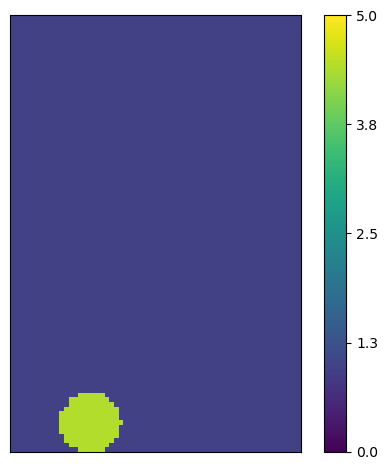
\includegraphics[totalheight=\nhghaloesheight]{Figures/softplus_halos/ex1/mutrue.png}
    \caption{\label{fig:haloes_true} True}
  \end{subfigure}
  %
  \begin{subfigure}[c]{\nhghaloeswidth}
  \centering    
    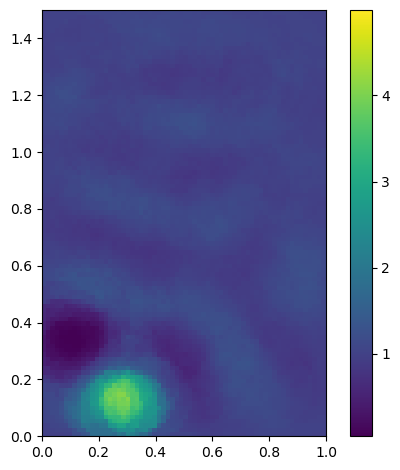
\includegraphics[totalheight=\nhghaloesheight]{Figures/softplus_halos/ex1/musoftplus.png}
    \caption{\label{fig:haloes_softplus} Softplus}
  \end{subfigure}
  %
  \begin{subfigure}[c]{\nhghaloeswidth}
    \centering
    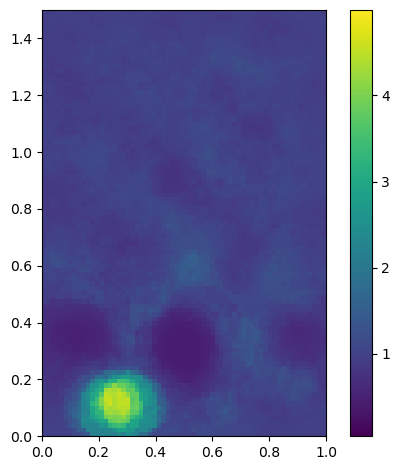
\includegraphics[totalheight=\nhghaloesheight]{Figures/softplus_halos/ex1/mutanhshiftp50.png}
    \caption{\label{fig:haloes_tanhp50} Twisted 1}            
  \end{subfigure}
  %
  \begin{subfigure}[c]{\nhghaloeswidth}
    \centering
    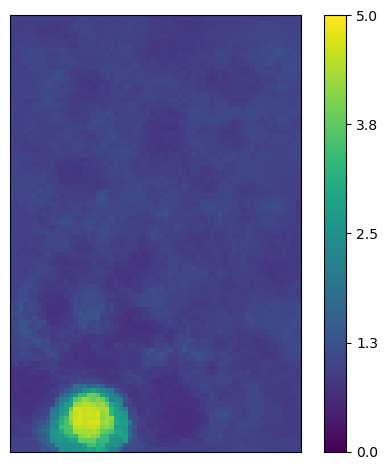
\includegraphics[totalheight=\nhghaloesheight]{Figures/softplus_halos/ex1/mutanhshiftp25.png}
    \caption{\label{fig:haloes_tanhp25} Twisted 2}        
  \end{subfigure}
  %
  \begin{subfigure}[c]{\nhghaloeswidth}
    \centering
    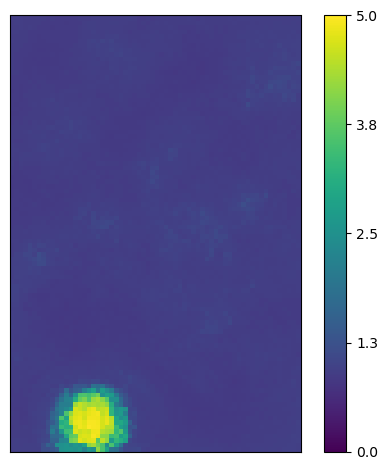
\includegraphics[totalheight=\nhghaloesheight]{Figures/softplus_halos/ex1/mutanhshift0.png}
    \caption{\label{fig:haloes_tanhp0} Twisted 3}    
  \end{subfigure}     
  %
  \caption{\label{fig:haloes} Reconstructions using the softplus activation function show regions of very low shear modulus (haloes), typically adjoining inclusions. Twisted 1, Twisted 2 and Twisted 3 correspond to the twisted tanh $[0.5, 5.5]$, twisted tanh $[0.75,5.25]$ and twisted tanh $[1.0,5.0]$ activations. The better our prior knowledge about the shear modulus, the lesser the haloes. These figures are on the same color scale. See also table (\ref{table:muminmax}).}
\end{figure}
%
\begin{table}
 \centering
 \begin{tabular}{|l|l|}
   \hline
   CNN Layer & Specifications \\
   \hline
   \multirow{3}{*}{conv2d}  & $32$ filters, kernel size $3$,\\ & activation is \textit{relu},\\& no regularization\\
   \hline
   max\_pooling2d: & pool size $2$, strides $2$\\
   \hline
   \multirow{3}{*}{conv2d\_1} & $64$ filters, kernel size $3$,\\& activation is \textit{relu},\\ & no regularization\\
   \hline
   max\_pooling2d\_1: & pool size $2$, strides $2$\\
   \hline
   flatten & -\\
   \hline
   \multirow{3}{*}{dense}  & $128$ units,\\& activation \textit{relu},\\& no regularization\\
   \hline
   \multirow{3}{*}{dense\_1} & $nnodex*nnodey$ units,\\& activation or twisted tanh,\\& no regularization\\
   \hline
 \end{tabular}
 \caption{\label{table:cnnlayerparams} Parameters for the CNN shown in figure (\ref{fig:typical_cnn}).}
\end{table}
%
\begin{figure}[!h] 
   \centering
    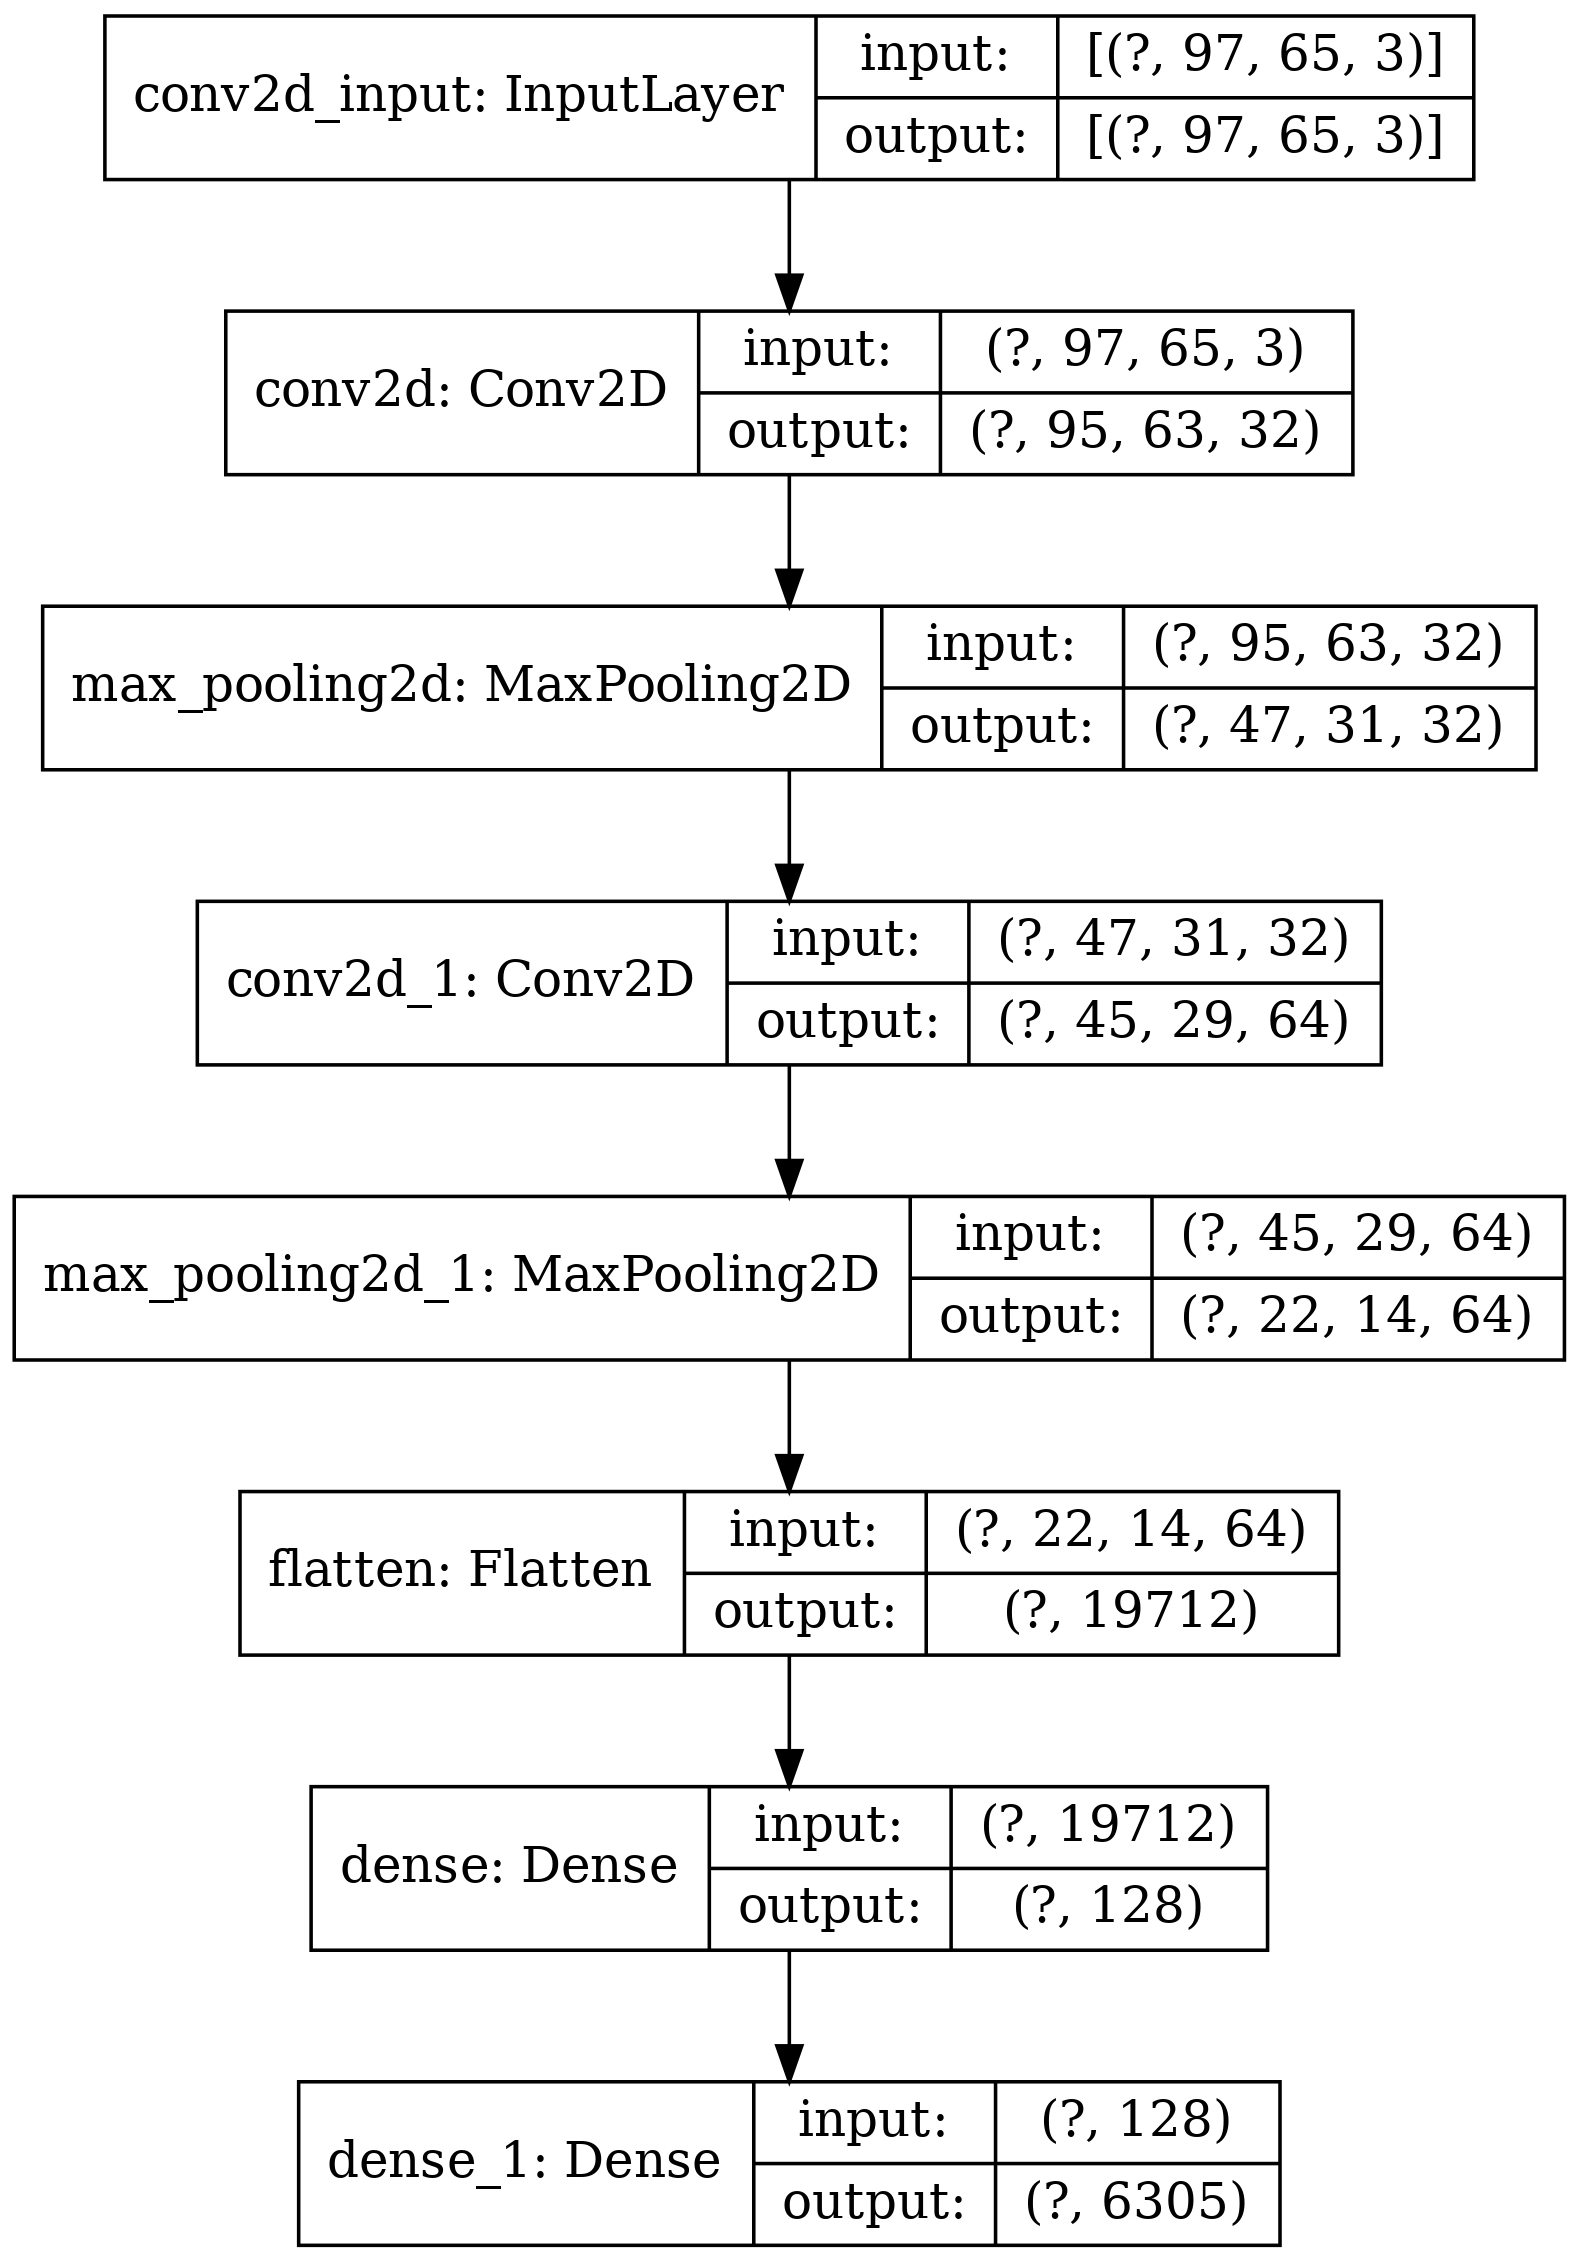
\includegraphics[totalheight=9cm]{Figures/typical_cnn.png}
    \caption{\label{fig:typical_cnn}Typical CNN architecture used in this work. This architecture is essentially the same the one used in the Deep Learning example in \cite{misc:udemy} in which it was used to classify images into two categories: 'cat' or 'dog'.}
\end{figure}
%
%
\section{Results}
We present results for the CNNs described in table (\ref{table:cnnparams}). Their architecture is given in figure (\ref{fig:typical_cnn}) and the layer parameters are given in table (\ref{table:cnnlayerparams}). Every CNN is trained for 384 epochs to put them on a equal footing for comparison. At $\approx{12}$ seconds per epoch, the network takes $\approx{1.5}$ hours to train. All CNNs use the twisted tanh $[0.75,5.25]$ activation. This means that we instruct the CNNs to predict shear moduli approximately in the range $[0.75,5.25]$ as opposed to the true range $[1.0,5.0]$. Thus, we are not assuming perfect knowledge of the upper and lower bounds for the shear modulus in the problem. We present the best and worst reconstructions, according to equation (\ref{eqn:scalederror}), and two other reconstructions which illustrate the performance of our neural network. We present additional supporting reconstructions in Appendix (\ref{sect:appendix1}).
\subsection{Error metrics}
We introduce new metrics, namely the \textit{inclusion scaled error} and \textit{background scaled error}, to evaluate the performance of the neural networks. These metrics  measure the average percentage error in the shear modulus in the background or in the inclusion. We define inclusion scaled error for the $i^{th}$ test example $\eta_{i}$ and its average $\eta_{ave}$ as
\begin{subequations}
  \begin{align}
  \eta_{i} &\coloneqq \frac{1}{n_{inc_i}}\sum_{j=1}^{n_{inc_i}}\frac{\mu^{i,predicted}_{j}-\mu^{i,true}_{j}}{\mu^{i,true}_{j}},  &\label{eqn:incscalederror}\\
  \eta_{ave} &\coloneqq \frac{\sum_{i=1}^{n_{test}}\eta_{i}}{n_{test}}. &\label{eqn:averageincscalederror}
  \end{align}
\end{subequations}
In the above equations, $\mu_{j}^{i,true}$ is the $j^{th}$ component of a vector $\mu^{i,true}$ containing true values of the shear modulus for the $i^{th}$ test example, \textit{restricted to the inclusion(s)} only. $\mu_{j}^{i,predicted}$ is the $j^{th}$ component of a vector $\mu^{i,predicted}$ containing corresponding predictions. $n_{inc_i}$ is the number of nodes in the inclusion(s) for the $i^{th}$ test example. $n_{test}$ is the number of test examples, in our case $800$. The quantities $\eta_i$ and $\eta_{ave}$ capture how accurately the shear modulus of the inclusions is predicted. Positive values of $\eta_i$ and $\eta_{ave}$ indicate over-prediction. Negative values indicate under-prediction.

The background scaled error $\xi_{i}$ and its average $\xi_{ave}$ can be defined similarly, by replacing $n_{inc_i}$ in equations (\ref{eqn:incscalederror}) and (\ref{eqn:averageincscalederror})  with $n_{back_i}$ (the number of nodes in the background) and restricting the vectors $\mu^{i,true}$ and $\mu^{i,predicted}$ to the background only.
%
\subsection{\label{sect:resultscnn1}Results for CNN1}
%
The training and validation losses for CNN1 are shown in figure (\ref{fig:cnn1losses}). The average inclusion scaled error is $-0.117$ and the average background scaled error is $-0.0171$. These indicate that, on average, the shear modulus of the inclusions is under-predicted. The background, on average, is predicted accurately.

Reconstructions are shown in figure (\ref{fig:cnn1result}). Figure (\ref{fig:cnn1resulta}) is our best result according to equation (\ref{eqn:scalederror}). The location and shear-modulus of the inclusion is predicted accurately. In figure (\ref{fig:cnn1resultc}) the location of multiple inclusions is predicted accurately but there is error in the stiffness. Figures (\ref{fig:cnn1resultb}-\ref{fig:cnn1resultd}) show that the inclusions having small size or low shear modulus are not accurately reconstructed. Their reconstruction can be best described as 'wisps'. We present additional supporting results in figure (\ref{fig:app1result}) in Appendix (\ref{sect:appendix1}).

Figure (\ref{fig:cnn1histo}) shows histograms in which the scaled error, equation (\ref{eqn:scalederror}), is on the x-axis and the y-axis represents the fraction of examples in each bin (number of examples in each bin divided by the total number of examples). It is seen that the examples appear to be normally distributed around a mean of ${0.207}$ with standard deviation $0.0531$ and that $80\%$ test examples have scaled error of less than $0.19$. The maximum and minimum shear moduli in the prediction are $5.32$ and $0.631$. 
% Losses for CNN1
\begin{figure}[!h]
  \centering
  \begin{subfigure}[c]{\nhghalfwidth}
    \centering
    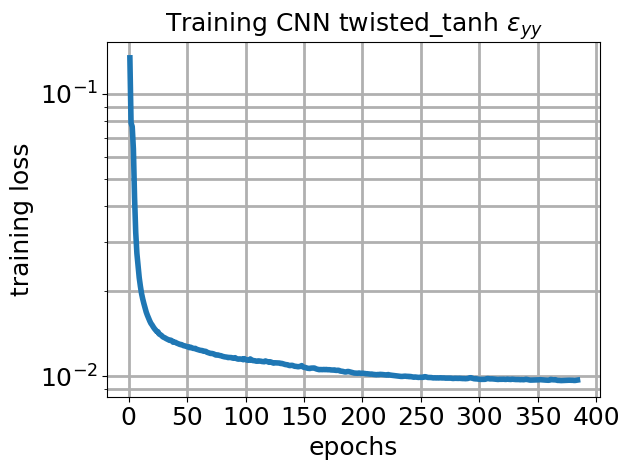
\includegraphics[totalheight=\nhgtotalheight]{Figures/Results1/loss.png}
    \subcaption{Loss}
  \end{subfigure}
%  
  \begin{subfigure}[c]{\nhghalfwidth}
    \centering    
    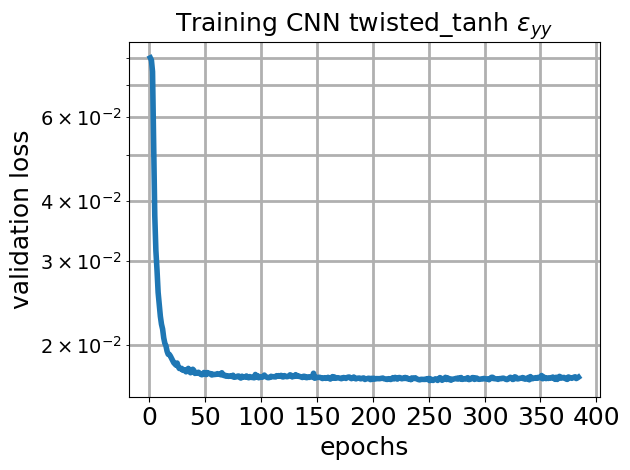
\includegraphics[totalheight=\nhgtotalheight]{Figures/Results1/val_loss.png}
    \subcaption{Validation loss}
  \end{subfigure}
  %
  \caption{\label{fig:cnn1losses} Training and validation losses for CNN1.}
\end{figure}
%
% Results for CNN1
\begin{figure}[!h]
  \centering
  \begin{subfigure}[c]{\nhghalfwidth}
    \centering
    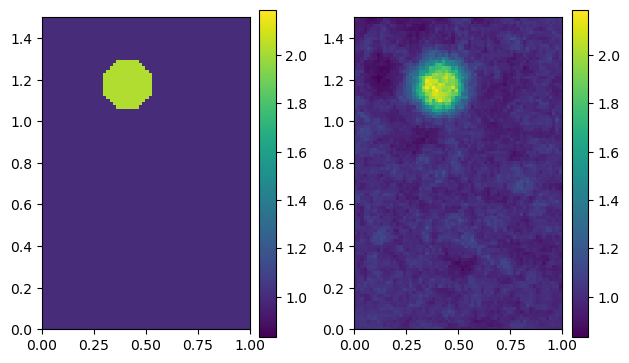
\includegraphics[totalheight=\nhgtotalheight]{Figures/Results1/ex1/mu.png}
    \subcaption{\label{fig:cnn1resulta}Best (0.0786)}
  \end{subfigure}
  %
  \begin{subfigure}[c]{\nhghalfwidth}
    \centering
    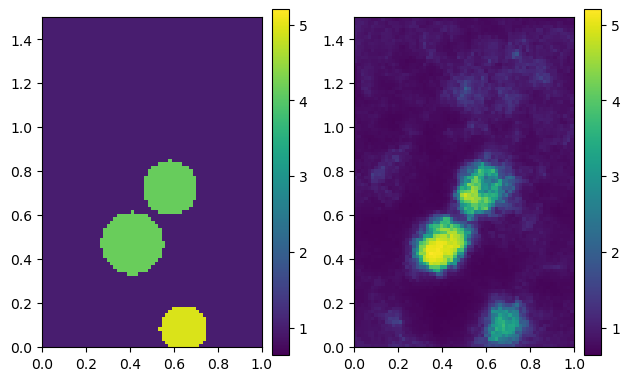
\includegraphics[totalheight=\nhgtotalheight]{Figures/Results1/ex2/mu.png}
    \subcaption{\label{fig:cnn1resultb}Worst (0.391)}
  \end{subfigure}
  %
  \begin{subfigure}[c]{\nhghalfwidth}
    \centering
    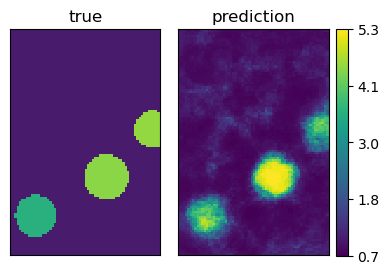
\includegraphics[totalheight=\nhgtotalheight]{Figures/Results1/ex3/mu.png}
    \subcaption{\label{fig:cnn1resultc}(0.286)}
  \end{subfigure}
  %
  \begin{subfigure}[c]{\nhghalfwidth}
    \centering
    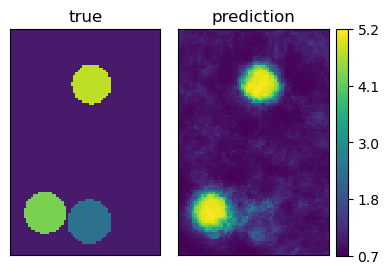
\includegraphics[totalheight=\nhgtotalheight]{Figures/Results1/ex4/mu.png}
    \subcaption{\label{fig:cnn1resultd}(0.252)}
  \end{subfigure}
\caption{\label{fig:cnn1result} Sample results for CNN1. The numbers in the brackets are the scaled errors as defined in equation (\ref{eqn:scalederror}).}  
\end{figure}
%
% Histograms for CNN1
\begin{figure}[!h]
\captionsetup[subfigure]{justification=centering}
  \centering
  \begin{subfigure}[c]{\nhghalfwidth}
    \centering
    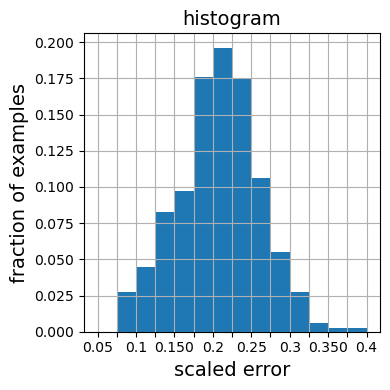
\includegraphics[totalheight=\nhgtotalheight]{Figures/Results1/histogram.png}
    \subcaption{Histogram}
  \end{subfigure}
%  
  \begin{subfigure}[c]{\nhghalfwidth}
    \centering
    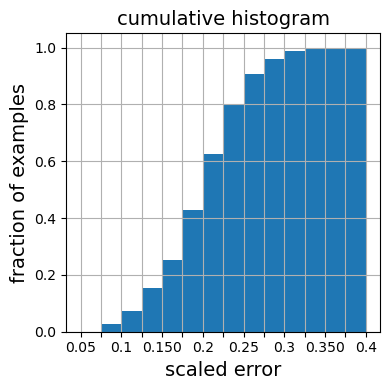
\includegraphics[totalheight=\nhgtotalheight]{Figures/Results1/cumulative.png}
    \subcaption{Cumulative histogram}
  \end{subfigure}
  %
  \caption{\label{fig:cnn1histo} Histogram and cumulative histogram for CNN1.}
\end{figure}
%
\subsection{\label{sect:resultscnn2}Results for CNN2}
The training and validation losses for CNN1 are shown in figure (\ref{fig:cnn2losses}). The average inclusion scaled error is $-0.123$ and the average background scaled error is $-0.0107$. These indicate that, on average, the shear modulus of the inclusions is under-predicted. The background, on average, is predicted accurately.

Figure (\ref{fig:cnn2resulta}) is our best result and shows accurate shear modulus and location prediction. In figure (\ref{fig:cnn2resultb}), the location of the inclusions is detected accurately, but not their shear modulus. As in section (\ref{sect:resultscnn1}), figures (\ref{fig:cnn2resultb}-\ref{fig:cnn2resultd}) show that the inclusions having low shear modulus or small size are not accurately reconstructed. Comparing figures (\ref{fig:cnn1resultc}) and (\ref{fig:cnn1resultd}) with figures (\ref{fig:cnn2resultc}) and (\ref{fig:cnn2resultd}) it appears that the displacement based neural network is better at reconstructing inclusions of small size and low shear modulus. We present supporting evidence in section (\ref{sect:discussion}). Finally, we present additional results illustrating the performance of the network in figure (\ref{fig:app2result}) in Appendix (\ref{sect:appendix1}).

As described before in section (\ref{sect:resultscnn1}), figure (\ref{fig:cnn2histo}) shows histograms of the scaled error. It is seen that the examples appear to be normally distributed around a mean of ${0.229}$ with standard deviation of $0.0552$ and that $65.8\%$ test examples have scaled error of less than $0.25$. This is much worse than the corresponding number ($80\%$)for CNN1, indicating that strain based CNNs perform better than displacement based CNNs. The maximum and minimum shear moduli in the prediction are $5.267$ and $0.643$. 
% Losses for CNN2
\begin{figure}[!h]
  \centering
  \begin{subfigure}[c]{\nhghalfwidth}
    \centering
    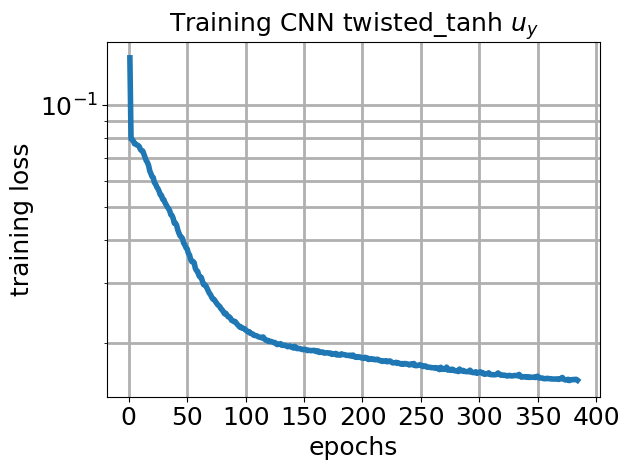
\includegraphics[totalheight=\nhgtotalheight]{Figures/Results2/loss.png}
    \subcaption{Loss}
  \end{subfigure}
%  
  \begin{subfigure}[c]{\nhghalfwidth}
    \centering
    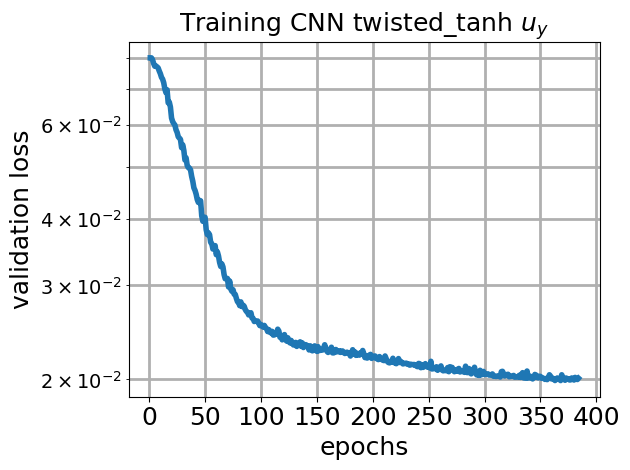
\includegraphics[totalheight=\nhgtotalheight]{Figures/Results2/val_loss.png}
    \subcaption{Validation loss}
  \end{subfigure}
  %
  \caption{\label{fig:cnn2losses} Training and validation losses for CNN2.}
\end{figure}
%
% Results for CNN2
\begin{figure}[!h]
  \centering
  \begin{subfigure}[c]{\nhghalfwidth}
    \centering
    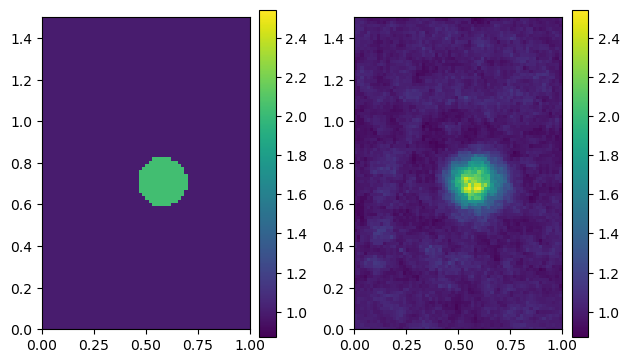
\includegraphics[totalheight=\nhgtotalheight]{Figures/Results2/ex1/mu.png}
    \subcaption{\label{fig:cnn2resulta}Best (0.0972)}
  \end{subfigure}
  %
  \begin{subfigure}[c]{\nhghalfwidth}
    \centering
    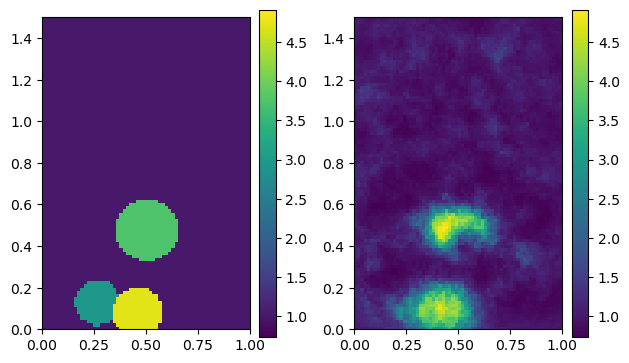
\includegraphics[totalheight=\nhgtotalheight]{Figures/Results2/ex2/mu.png}
    \subcaption{\label{fig:cnn2resultb}Worst (0.494)}
  \end{subfigure}
  %
  \begin{subfigure}[c]{\nhghalfwidth}
    \centering
    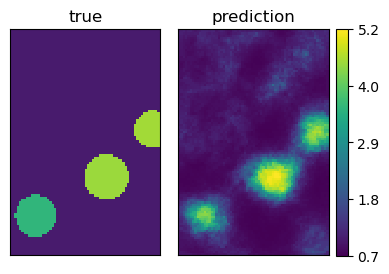
\includegraphics[totalheight=\nhgtotalheight]{Figures/Results2/ex3/mu.png}
    \subcaption{\label{fig:cnn2resultc}(0.308)}
  \end{subfigure}
  %
  \begin{subfigure}[c]{\nhghalfwidth}
    \centering
    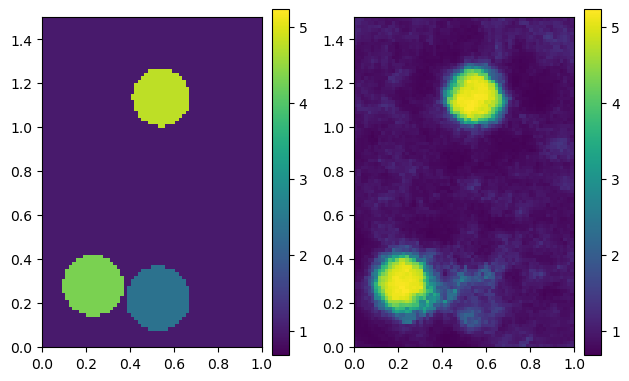
\includegraphics[totalheight=\nhgtotalheight]{Figures/Results2/ex4/mu.png}
    \subcaption{\label{fig:cnn2resultd}(0.279)}
  \end{subfigure}
\caption{\label{fig:cnn2result} Sample results for CNN2. The numbers in the brackets are the scaled errors as defined in equation (\ref{eqn:scalederror}). Figures (c) and (d) are the same test examples presented in figures (\ref{fig:cnn1resultc}) and (\ref{fig:cnn2resultd}).}  
\end{figure}
%
% Histograms for CNN2
\begin{figure}[!h]
\captionsetup[subfigure]{justification=centering}
  \centering
  \begin{subfigure}[c]{\nhghalfwidth}
    \centering
    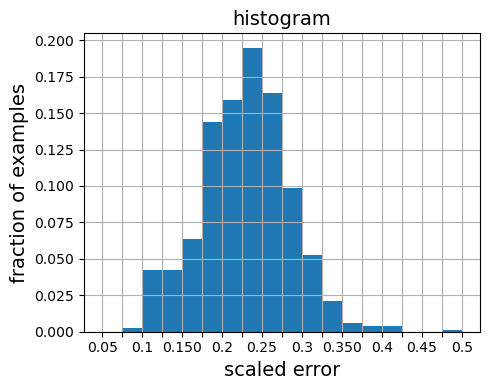
\includegraphics[totalheight=\nhgtotalheight]{Figures/Results2/histogram.png}
    \subcaption{Histogram}
  \end{subfigure}
%  
  \begin{subfigure}[c]{\nhghalfwidth}
    \centering
    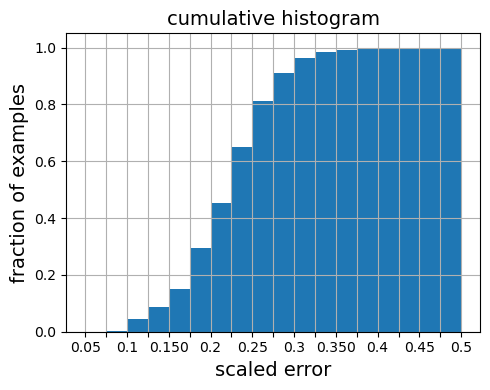
\includegraphics[totalheight=\nhgtotalheight]{Figures/Results2/cumulative.png}
    \subcaption{Cumulative histogram}
  \end{subfigure}
  %
  \caption{\label{fig:cnn2histo} Histogram and cumulative histogram for CNN2.}
\end{figure}
%
\subsection{\label{sect:resultscnn3}Results for CNN3}
In this section, we evaluate the ability of the CNN to generalize to the type of examples outside its training set. As noted in table (\ref{table:cnnparams}) we train the CNN using data which was generated using only one inclusion. But we evaluate it on data containing one, two or three inclusions.

Figure (\ref{fig:cnn3resulta}) shows accurate prediction of the shear modulus and location of the inclusion. This is not surprising because this example lies within the training space of the inclusion. The under-prediction of the inclusion stiffness is more severe than the results for CNN1 and CNN2. In figure (\ref{fig:cnn3resultb}) the inclusion on the lower right is completely missed. The size of the inclusions on the upper right is severely under-predicted. In figures (\ref{fig:cnn3resultc}) and (\ref{fig:cnn3resultd}), we see the inclusions with higher shear modulus being accurately predicted and the inclusions with low shear modulus being predicted as wisps. However, in spite of being trained on data containing a single inclusion, the network detects two out of three inclusions. As before, the inclusions with the lowest shear modulus are detected as wisps. Figures (\ref{fig:cnn3resultc}) and (\ref{fig:cnn3resultd}) indicate that the network has some ability to generalize to unseen examples. Finally, we present additional results illustrating the performance of the network in figure (\ref{fig:app3result}) in Appendix (\ref{sect:appendix1}).

The training and validation losses for CNN3 are shown in figure (\ref{fig:cnn3losses}). The average inclusion scaled error is $-0.187$ and the average background scaled error is $-0.0367$. These indicate that, on average, the shear modulus of the inclusions is under-predicted, and that of the background is predicted accurately.

As described before in section (\ref{sect:resultscnn1}), figure (\ref{fig:cnn3histo}) shows histograms of the scaled error. It is seen that the examples appear to be normally distributed around a mean of ${0.229}$ which is only slightly worse than CNN1 and CNN2. The standard deviation is $0.0727$ which is significantly higher than CNN1 and CNN2. $62.8\%$ examples have a scaled error less that $0.25$. This is much worse than the corresponding number for CNN1 ($80\%$) indicating that CNNs do not generalize perfectly. The maximum and minimum shear moduli in the prediction are $5.37$ and $0.513$.

% Losses for CNN3
\begin{figure}[!h]
  \centering
  \begin{subfigure}[c]{\nhghalfwidth}
    \centering
    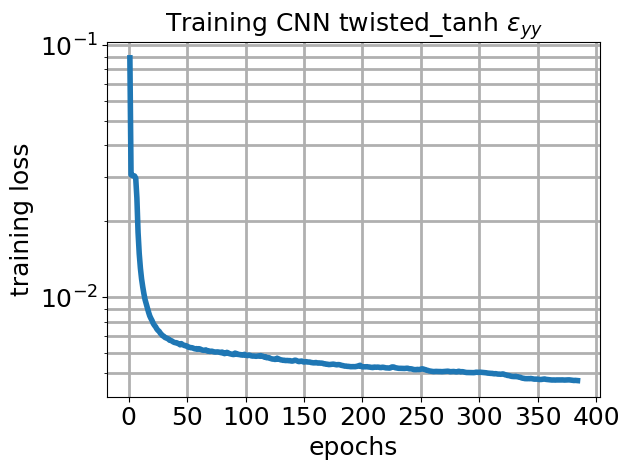
\includegraphics[totalheight=\nhgtotalheight]{Figures/Results3/loss.png}
    \subcaption{Loss}
  \end{subfigure}
%  
  \begin{subfigure}[c]{\nhghalfwidth}
    \centering
    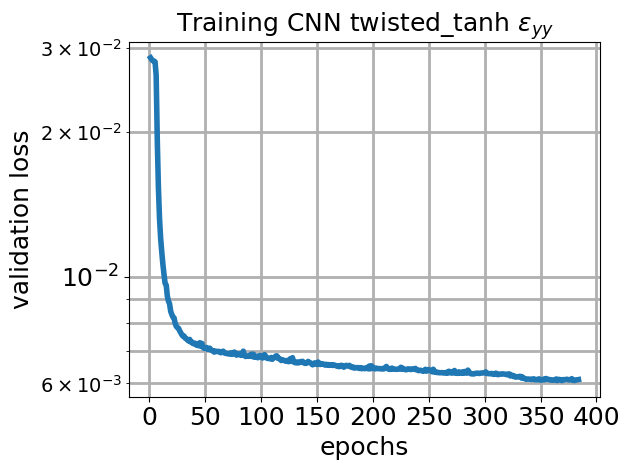
\includegraphics[totalheight=\nhgtotalheight]{Figures/Results3/val_loss.png}
   \subcaption{Validation loss}
  \end{subfigure}
  %
  \caption{\label{fig:cnn3losses} Training and validation losses for CNN3.}
\end{figure}
%
% Results for CNN3
\begin{figure}[!h]
  \centering
  \begin{subfigure}[c]{\nhghalfwidth}
    \centering    
    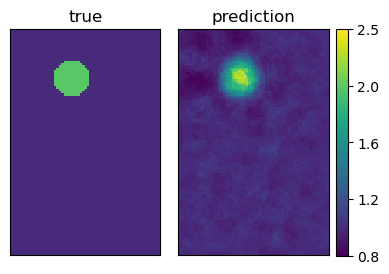
\includegraphics[totalheight=\nhgtotalheight]{Figures/Results3/ex1/mu.png}
    \subcaption{\label{fig:cnn3resulta}Best (0.0769)}
  \end{subfigure}
  %
  \begin{subfigure}[c]{\nhghalfwidth}
    \centering    
    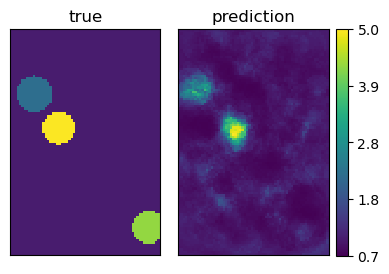
\includegraphics[totalheight=\nhgtotalheight]{Figures/Results3/ex2/mu.png}
    \subcaption{\label{fig:cnn3resultb}Worst (0.497)}
  \end{subfigure}
  %
  \begin{subfigure}[c]{\nhghalfwidth}
    \centering
    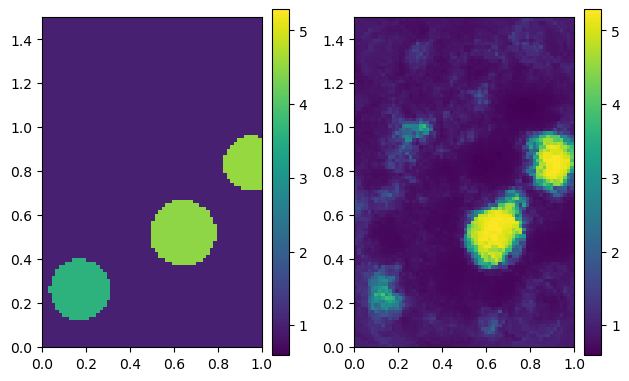
\includegraphics[totalheight=\nhgtotalheight]{Figures/Results3/ex3/mu.png}
    \subcaption{\label{fig:cnn3resultc}(0.397)}
  \end{subfigure}
  %
  \begin{subfigure}[c]{\nhghalfwidth}
    \centering
    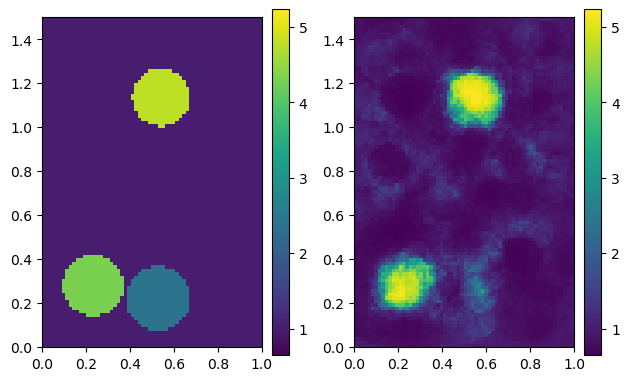
\includegraphics[totalheight=\nhgtotalheight]{Figures/Results3/ex4/mu.png}
    \subcaption{\label{fig:cnn3resultd}(0.303)}
  \end{subfigure}
\caption{\label{fig:cnn3result} Sample results for CNN3. The numbers in the brackets are the scaled errors as defined in equation (\ref{eqn:scalederror}). Figures (c) and (d) are the same test examples presented in figures (c) and (d) of figures (\ref{fig:cnn1result}) and (\ref{fig:cnn2result}) respectively.}  
\end{figure}
%
% Histograms for CNN3
\begin{figure}[!h]
\captionsetup[subfigure]{justification=centering}
  \centering
  \begin{subfigure}[c]{\nhghalfwidth}
    \centering
    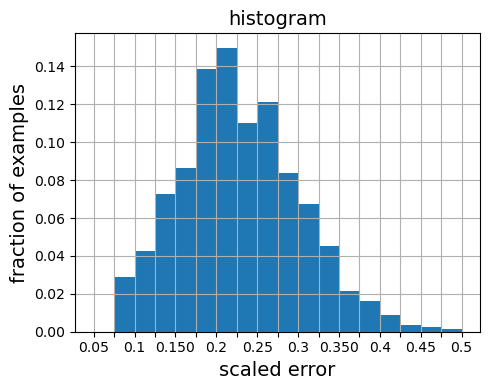
\includegraphics[totalheight=\nhgtotalheight]{Figures/Results3/histogram.png}
    \subcaption{Histogram}
  \end{subfigure}
%  
  \begin{subfigure}[c]{\nhghalfwidth}
      \centering
    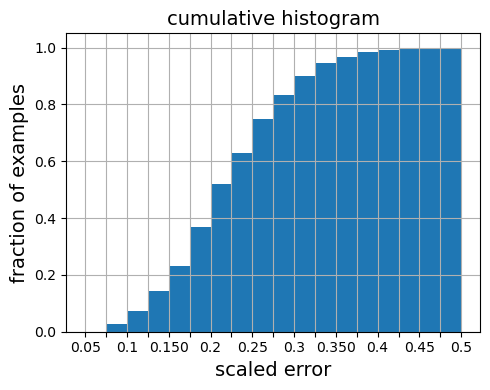
\includegraphics[totalheight=\nhgtotalheight]{Figures/Results3/cumulative.png}
    \subcaption{Cumulative histogram}
  \end{subfigure}
  %
  \caption{\label{fig:cnn3histo} Histogram and cumulative histogram for CNN3.}
\end{figure}
%
\subsection{\label{sect:discussion}Discussion}
We observe encouraging results with good qualitative agreement between the true and predicted shear shear modulus images. The average error according to equation (\ref{eqn:averagescalederror}) is seen to be $\approx{20\%}$. The shear modulus of inclusions is under-predicted. The shear modulus of inclusions with low shear modulus and small sized inclusions is significantly under-predicted. The average inclusion scaled error, equation (\ref{eqn:averageincscalederror}) evaluated over inclusions having shear modulus in the range $[2.0,3.0]$ yields $-0.151,-0.113$ and $-0.224$ for CNN1, CNN2 and CNN3 respectively. This shows that the strain based networks CNN1 and CNN3 perform worse than usual while detecting inclusions which whose shear modulus is low. The displacement based network CNN2 does not appear to degrade. Its performance while detecting inclusions of low shear modulus is comparable to its performance while detecting inclusions of relatively high shear modulus. Table (\ref{table:cnnstatsummary}) summarizes the performance of the three CNNs evaluated in this work. 

% CNN1 - 2-3norm - -0.151
% CNN2 - 2-3norm - -0.113
% CNN3 - 2-3norm - -0.224

\begin{table}
  \centering
  \begin{tabular}{|c|c|c|}
    \hline
    \multirow{2}{*}{CNN Name} & Average scaled & Average inclusion \\
                              & scaled error   & scaled error      \\
    \hline
    CNN1     & 0.207 & -0.117\\
    \hline
    CNN2     & 0.229 & -0.123\\
    \hline
    CNN3     & 0.229 & -0.187\\
    \hline
  \end{tabular}
  \caption{\label{table:cnnstatsummary} Errors for the CNNs considered.}
\end{table}  

We see that the axial strain based neural network (section {\ref{sect:resultscnn1}}) outperforms the axial displacement based network (section \ref{sect:resultscnn2}). We think that exploring the physical meaning of the convolutional filters learned using Fourier analysis as in \cite{paper:pateloberai2019} is a promising direction for investigating the reason for out-performance. The results presented in section (\ref{sect:resultscnn3}) figures (\ref{fig:cnn3resultc}) and (\ref{fig:cnn3resultd}) show that the network has some ability to generalize to unseen examples.
%
\section{Concluding remarks}
% Custom activation function
% https://stackoverflow.com/questions/43915482/how-do-you-create-a-custom-activation-function-with-keras
In this work, we have presented CNNs capable of predicting shear modulus fields from displacement or strain fields. We used the twisted tanh function as the activation function of the output layer. We observed that with appropriate prior knowledge about the minimum and maximum shear modulus in the problem, the twisted tanh activation function reduces the incidence of 'haloes' (regions of low shear modulus) around the inclusions. The shear modulus of the inclusions with shear modulus close to the background modulus, or small inclusions, was predicted as wisps, while regions of high shear modulus were predicted more accurately.    
\subsection{Directions for future work}
\begin{enumerate}
\item{Addition of homogeneous examples to the dataset would be a good test for the CNNs evaluated in this work However, given that the CNNs under-predict the shear modulus of small inclusions, we believe homogeneous examples will be predicted correctly.}
\item{Training the CNN with displacement or strain data generated using random values for the shear modulus at each node and seeing if it learns the inverse operator from the displacement (or strain) fields to shear modulus fields would be interesting. Training with other complex shapes for the shear modulus would also be interesting.}
\item{Training with examples in which shear modulus of only one node is changed relative to the background. It would be interesting, if based on this information, the CNN can process a displacement field and understand that the stiffness of only certain nodes needs to be changed.}
\item{It is seen that better results are obtained for larger inclusion with larger contrast. Stiffness of smaller inclusions is under-predicted. Designing a network to accurately image small inclusions will be interesting. We note that having material properties and displacements on the same mesh may lead to unconverged displacements for smaller inclusions. These unconverged displacements will not have enough features/information to be able to predict stiffness fields from them. It may be useful to make the displacement mesh much finer than the shear modulus mesh so as to resolve features created by small inclusions. We also note that from previous experience, the adjoint method \cite{paper:oberai2003,paper:gokhale2008,paper:goenezen2011} is able to predict the small inclusions correctly using noiseless data. It appears that the adjoint method does better than CNNs on the problem of predicting small inclusions.}
\item{We think that Fourier analysis of these filters, as reported in \cite{paper:pateloberai2019} would be valuable. Using their technique, we can identify some filters with the derivative in the $x$ or $y$ direction, but the physical meaning of the majority of filters is not clear. We belive that after understanding the physical meaning of each filter, better filters could perhaps be constructed manually. On a related note, visualization of intermediate images produced by the convolutional layers is also a promising direction.}
\item{We have trained the CNN using examples in which the stiffness of the circular inclusion lies between $2.0$ and $5.0$. We call this the training range. The test data also contains examples in the \textit{same} range. Expanding this test range to include examples outside the training range and evaluating the performance of the CNNs will be interesting. We note that we have tested the ability of the CNN to generalize beyond its training set in section (\ref{sect:resultscnn3}), where a CNN trained only one inclusion in its training examples was evaluated on data containing one to three inclusions. We obtained reasonable performance in this case.}
\item{A simple \textit{mean squared error} (which corresponds to the square of the $L^2$ norm in the continuous case) was used to evaluate the loss function for the neural network. The effect of other losses corresponding to $H^1$ or Total Variation Diminishing (TVD) norms will be interesting to evaluate. We think that, based on our experience \cite{diss:gokhale2007}, using a loss function corresponding to the $H^1$ norm will remove the incidence of regions of low shear modulus adjacent to inclusions. However, it will also penalize sharp discontinuities in the inclusions as well. If we are training with both components of a noiseless displacement field, then one can consider a loss function which is simply the residual obtained when the predicted shear modulus and input fields are plugged into the equilibrium equations of elasticity. Implementing these loss functions will require custom loss functions in TensorFlow perhaps along with custom gradient calculation.}
\item{Investigating different network architectures with the aim of yielding better results will be worth investigating. More CNN layers (or less), deeper (or shallower) networks, should be investigated. Other hyperparameters, such as the kernel size for the CNN layers, can be varied as well. It may be worth investigating whether a CNN is required at all and whether a simple dense network can produce similar quality results. The first dense layer contains $128$ nodes. Increasing this number will probably result in better networks, but will also increase the number of weights and hence training time. It may also be worthwhile to replace the full connection of the dense layers with spatially close connections. By this, we mean that after flattening each node in the first dense layer would be connected only to those neurons which are spatially close together in the previous layer.}
\item{Medical image registration to obtain a displacement field is a difficult process. It would be an important advance if we could train neural networks to work directly with medical images instead of the computed displacement field. This would involve training the CNN by computing thousands of displacement fields by hand and solving an inverse problem and using the predicted shear modulus field as labeled data as input to the CNN. Additional information could be obtained by doctors interpreting medical images and identifying tumors and their mechanical properties.}
\item{Since the initial choices for the CNN weights are random, we can train the network multiple times and get different values for the network weights. Having thus obtained many CNNs with different weights, we are led to the following two options. One, we can average the weights of the CNNs to obtain an averaged network. Two, we can make multiple predictions with the different CNNs and then average the result. The second option will require large storage because CNNs have millions of parameters. These options should be investigated.}
\item{It would be interesting to consider a multiscale/hierarchical neural network. This neural network would first make a prediction of the average shear modulus field using only a few weights. In the next step, more nodes would be introduced and, say, 9 nodes would be introduced to make a prediction of the shear modulus field. The number of layers and neurons would be increased and the weights would be initialized from the previous neural network. This process can continue until a neural network which can make detailed predictions of the stiffness field can be obtained.}
\item{In this work, CNNs were trained on noiseless data and then used to make predictions on noisy data. Another option could be to increase the number of training set examples by adding noise to them and see whether the predictions become more accurate. This can dramatically increase the size of the training set.}
\item{Extending this work to actual complex three dimensional organ geometries discretized using unstructured finite element meshes will be interesting because the domain will no longer be rectangular. Evaluating loss functions on finite element meshes will require custom loss functions. Another method that could be considered is to approximate the organ geometry using a structured grid. That is, if the center of the cell lies inside the organ, then that entire cell is considered to be inside the organ. Cells outside the organ can have placeholder data, while cells inside the organ can have actual displacement or strain data. Because the geometry is now represented on a structured grid, simple CNNs can be used. We believe that while this method may be feasible in two dimensions, it will result in a waste of storage space in three dimensions.}
\item{Multiple displacement fields: In \cite{paper:barbonegokhale,paper:barbonebamber} the authors show that a single strain or displacement field is not sufficient to predict the shear modulus field uniquely and multiple displacement fields are required for unique prediction of the shear modulus field. The use of multiple displacement fields can be considered within our current framework by increasing the number of channels the input images. See Section (\ref{sect:cnnarch}).} 
\item{Assuming that inclusions are roughly circular, several auxiliary problems may be considered. Given a displacement field, strain field or shear modulus field (computed by any inversion procedure) one may train a CNN to compute : 1) Whether or not an inclusion or inclusions exist  in the domain. This is the \textit{binary classification problem}. Our experience with this suggests that this problem can be solved accurately in the absence of noise.  Adding noise to the data and using a CNN trained on noisy data to make this prediction results in inaccurate results. 2) The number of inclusions in the problem 3) The shear modulus of each inclusion 4) The location of the center of each inclusion 5) The radius of each inclusion.}
\item{Enforcing constraints on the shear modulus is easy in traditional iterative methods. We just supply bound constraints to the optimization algorithm. On the other hand, for the type of problem studied in this work, constraints on the shear modulus values result in constraints on the activation function of the final output layer, and not on the input variables. Applying bound constraints to the shear modulus is hard and requires the use of special activation functions which may get stuck in a local minimum. This problem has been alleviated to a large extent by the use of the twisted tanh activation function. Finally we note that one can solve a non-linearly constrained optimization problem to train the neural network in which the output of the final layer is constrained between allowable values of the shear modulus. However, when an unseen example from the test set is presented, it is not possible to guarantee that this constraint will be satisfied.}
\item{A hybrid approach combining machine learning and traditional approaches (iterative or direct) will be interesting. We envision that the ML based approach will provide a measure of the confidence in its output. If this is confidence is low, then a solution will be computed using traditional methods and perhaps added to the machine learning training dataset.}
\item{Extending the method studied in this document to predict multiple parameter fields will be interesting, because the method will have to study the features in the displacement or strain fields and then decide which parameter field was responsible for producing those features. Such cases will occur when we try to predict both $\lambda(x)$ and $\mu(x)$ for linear elasticity both the nonlinear parameter $\gamma(x)$ and the linear parameter $\mu(x)$ as in \cite{paper:gokhale2008}}.
\item{Software and performance issues: The finite element solver and associated scripts for generating and post-processing the data were written in Python 3.8. While the elements were accelerated using Numba \cite{conf:numba}, we believe that better performance could be obtained by writing the solver in C/C++/Fortran or Julia or using open source solvers like FEniCS \cite{paper:fenics} or deal.II \cite{paper:deal.ii}. Each FE input file is 3.3MB and output file is 1.1MB and total dataset size is $\approx$  20GB. Approximately 10 seconds were required to compute one training example. There was no effort made to minimize the size of input and output files. Simple text based JSON files were used because of their simplicity. If one wants increase the number of training examples by a factor of thousand, 20TB of data would be required. Optimized data structures and hardware supporting fast disk access (SSDs) will be necessary for scaling to large data sets. The use of GPU clusters to process large amounts of data may also need to be considered. The simulations to generate data and the CNN training in this work were carried out on an Intel i5-4460 3.2Ghz processor with four physical and logical cores and 8GB RAM. The OS used was Windows 10 running WSL2. TensorFlow 2.4 was used.}
\end{enumerate}
%\clearpage
\begin{appendices}
\section{\label{sect:appendix1} Additional supporting results}
We present additional supporting results in figures (\ref{fig:app1result}),(\ref{fig:app2result}) and (\ref{fig:app3result}) in order to provide a better sampling of the results produced by CNN1,CNN2 and CNN3.
%\subsection{Additional results for CNN1}
% Additional results for CNN1
\begin{figure}[!h]
  \centering
  %
  \begin{subfigure}[c]{\nhgappwidth}
    \centering    
    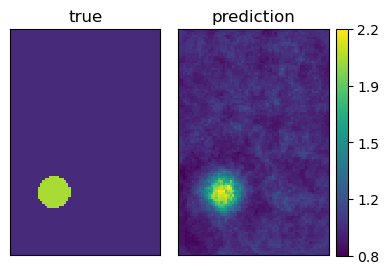
\includegraphics[totalheight=\nhgappheight]{Figures/Appendix/CNN1/ex1/mu.png}
    \subcaption{\label{fig:app1resulta} (0.0812)}
  \end{subfigure}
  %
  \begin{subfigure}[c]{\nhgappwidth}
    \centering    
    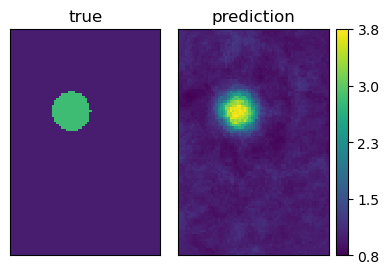
\includegraphics[totalheight=\nhgappheight]{Figures/Appendix/CNN1/ex2/mu.png}
    \subcaption{\label{fig:app1resultb} (0.142)}
  \end{subfigure}
  %
  \begin{subfigure}[c]{\nhgappwidth}
    \centering
    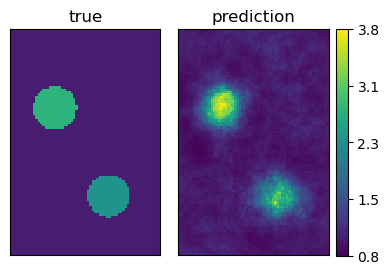
\includegraphics[totalheight=\nhgappheight]{Figures/Appendix/CNN1/ex3/mu.png}
    \subcaption{\label{fig:app1resultc}(0.174)}
  \end{subfigure}
  %
  \begin{subfigure}[c]{\nhgappwidth}
    \centering
    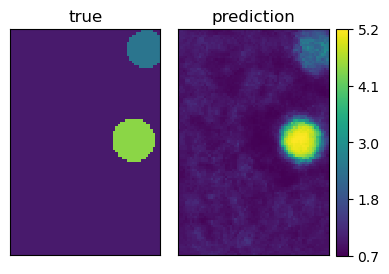
\includegraphics[totalheight=\nhgappheight]{Figures/Appendix/CNN1/ex4/mu.png}
    \subcaption{\label{fig:app1resultd}(0.191)}
  \end{subfigure}
    \begin{subfigure}[c]{\nhgappwidth}
    \centering    
    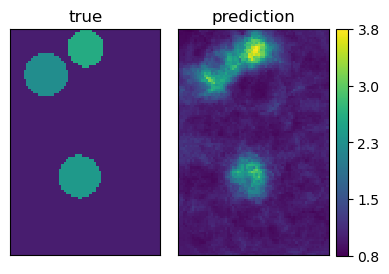
\includegraphics[totalheight=\nhgappheight]{Figures/Appendix/CNN1/ex5/mu.png}
    \subcaption{\label{fig:app1resulte} (0.208)}
  \end{subfigure}
  %
  \begin{subfigure}[c]{\nhgappwidth}
    \centering    
    \includegraphics[totalheight=\nhgappheight]{Figures/Appendix/CNN1/ex6/mu.png}
    \subcaption{\label{fig:app1resultf} (0.225)}
  \end{subfigure}
  %
  \begin{subfigure}[c]{\nhgappwidth}
    \centering
    \includegraphics[totalheight=\nhgappheight]{Figures/Appendix/CNN1/ex7/mu.png}
    \subcaption{\label{fig:app1resultg}(0.243)}
  \end{subfigure}
  %
  \begin{subfigure}[c]{\nhgappwidth}
    \centering
    \includegraphics[totalheight=\nhgappheight]{Figures/Appendix/CNN1/ex8/mu.png}
    \subcaption{\label{fig:app1resulth}(0.264)}
  \end{subfigure}
\caption{\label{fig:app1result} Additional results for CNN1. The numbers in the brackets are the scaled errors as defined in equation (\ref{eqn:scalederror}).}  
\end{figure}
%
%\subsection{Additional results for CNN2}
% Additional results for CNN2
\begin{figure}[!h]
  \centering
  %
  \begin{subfigure}[c]{\nhgappwidth}
    \centering    
    \includegraphics[totalheight=\nhgappheight]{Figures/Appendix/CNN2/ex1/mu.png}
    \subcaption{\label{fig:app2resulta} (0.0993)}
  \end{subfigure}
  %
  \begin{subfigure}[c]{\nhgappwidth}
    \centering    
    \includegraphics[totalheight=\nhgappheight]{Figures/Appendix/CNN2/ex2/mu.png}
    \subcaption{\label{fig:app2resultb} (0.164)}
  \end{subfigure}
  %
  \begin{subfigure}[c]{\nhgappwidth}
    \centering
    \includegraphics[totalheight=\nhgappheight]{Figures/Appendix/CNN2/ex3/mu.png}
    \subcaption{\label{fig:app2resultc}(0.193)}
  \end{subfigure}
  %
  \begin{subfigure}[c]{\nhgappwidth}
    \centering
    \includegraphics[totalheight=\nhgappheight]{Figures/Appendix/CNN2/ex4/mu.png}
    \subcaption{\label{fig:app2resultd}(0.213)}
  \end{subfigure}
    \begin{subfigure}[c]{\nhgappwidth}
    \centering    
    \includegraphics[totalheight=\nhgappheight]{Figures/Appendix/CNN2/ex5/mu.png}
    \subcaption{\label{fig:app2resulte} (0.231)}
  \end{subfigure}
  %
  \begin{subfigure}[c]{\nhgappwidth}
    \centering    
    \includegraphics[totalheight=\nhgappheight]{Figures/Appendix/CNN2/ex6/mu.png}
    \subcaption{\label{fig:app2resultf} (0.245)}
  \end{subfigure}
  %
  \begin{subfigure}[c]{\nhgappwidth}
    \centering
    \includegraphics[totalheight=\nhgappheight]{Figures/Appendix/CNN2/ex7/mu.png}
    \subcaption{\label{fig:app2resultg}(0.265)}
  \end{subfigure}
  %
  \begin{subfigure}[c]{\nhgappwidth}
    \centering
    \includegraphics[totalheight=\nhgappheight]{Figures/Appendix/CNN2/ex8/mu.png}
    \subcaption{\label{fig:app2resulth}(0.290)}
  \end{subfigure}
\caption{\label{fig:app2result} Additional results for CNN2. The numbers in the brackets are the scaled errors as defined in equation (\ref{eqn:scalederror}).}  
\end{figure}
%
%\subsection{Additional results for CNN3}
% Additional results for CNN3
\begin{figure}[!h]
  \centering
  %
  \begin{subfigure}[c]{\nhgappwidth}
    \centering    
    \includegraphics[totalheight=\nhgappheight]{Figures/Appendix/CNN3/ex1/mu.png}
    \subcaption{\label{fig:app3resulta} (0.0784)}
  \end{subfigure}
  %
  \begin{subfigure}[c]{\nhgappwidth}
    \centering    
    \includegraphics[totalheight=\nhgappheight]{Figures/Appendix/CNN3/ex2/mu.png}
    \subcaption{\label{fig:app3resultb} (0.144)}
  \end{subfigure}
  %
  \begin{subfigure}[c]{\nhgappwidth}
    \centering
    \includegraphics[totalheight=\nhgappheight]{Figures/Appendix/CNN3/ex3/mu.png}
    \subcaption{\label{fig:app3resultc} (0.179)}
  \end{subfigure}
  %
  \begin{subfigure}[c]{\nhgappwidth}
    \centering
    \includegraphics[totalheight=\nhgappheight]{Figures/Appendix/CNN3/ex4/mu.png}
    \subcaption{\label{fig:app3resultd}(0.201)}
  \end{subfigure}
    \begin{subfigure}[c]{\nhgappwidth}
    \centering    
    \includegraphics[totalheight=\nhgappheight]{Figures/Appendix/CNN3/ex5/mu.png}
    \subcaption{\label{fig:app3resulte} (0.222)}
  \end{subfigure}
  %
  \begin{subfigure}[c]{\nhgappwidth}
    \centering    
    \includegraphics[totalheight=\nhgappheight]{Figures/Appendix/CNN3/ex6/mu.png}
    \subcaption{\label{fig:app3resultf} (0.248)}
  \end{subfigure}
  %
  \begin{subfigure}[c]{\nhgappwidth}
    \centering
    \includegraphics[totalheight=\nhgappheight]{Figures/Appendix/CNN3/ex7/mu.png}
    \subcaption{\label{fig:app3resultg}(0.275)}
  \end{subfigure}
  %
  \begin{subfigure}[c]{\nhgappwidth}
    \centering
    \includegraphics[totalheight=\nhgappheight]{Figures/Appendix/CNN3/ex8/mu.png}
    \subcaption{\label{fig:app3resulth}(0.313)}
  \end{subfigure}
\caption{\label{fig:app3result} Additional results for CNN3. The numbers in the brackets are the scaled errors as defined in equation (\ref{eqn:scalederror}).}  
\end{figure}
%
\end{appendices}
\clearpage
\bibliography{eibib}{}
\bibliographystyle{plain}
\end{document}
%
% Document ends here
\appendix
\section{\label{sect:filters}Filters}
\subsection{\label{sect:filtcnn1}Filters for CNN1}
% solves 'Counter too large' problem
\renewcommand*{\thesubfigure}{\arabic{subfigure}}
\begin{figure}[!h]
  \filterpics{FiltersTanhStrain3}
  \caption{Filters for case 1}
\end{figure}  
\subsection{Filters for CNN2}
\begin{figure}[!h]
  \filterpics{FiltersTanhDisp3}
  \caption{Filters for case 2}
\end{figure}  
\subsection{Filters for CNN3}
\begin{figure}[!h]
  \filterpics{FiltersTanhStrain1}
  \caption{Filters for case 3}
\end{figure}  

